\documentclass[10pt]{beamer} 
\usetheme[pageofpages=of,% String used between the current page and the
          % total page count.
          alternativetitlepage=true,% Use the fancy title page.
          %titlepagelogo=coca,% Logo for the first page.
          titleline=true
          ]{Torino}
%\usetheme{Frankfurt}

\usecolortheme{chameleon}

\usepackage{graphicx,hyperref,url}
\usepackage[utf8]{inputenc}
\usepackage[T1]{fontenc}
\usepackage[portuges,brazilian]{babel}

\usepackage{caption}
\usepackage{subfigure}
%\usepackage{subcaption}
\usepackage{latexsym}
\usepackage{amssymb, amsmath}
\usepackage{multicol}
\usepackage{pifont}%,bbding}%%,dingbat} %%% ver manual de simbolos
\usepackage[final]{listings}
\usepackage{comment}
\usepackage{sansmathaccent}
\pdfmapfile{+sansmathaccent.map}

\definecolor{azulclaro}{rgb}{0.9,0.9,0.9}
\definecolor{mygreen}{rgb}{0,0.6,0}
\definecolor{mygray}{rgb}{0.5,0.5,0.5}
\definecolor{mymauve}{rgb}{0.58,0,0.82}
\definecolor{darkgray}{rgb}{.4,.4,.4}
\definecolor{purple}{rgb}{0.65, 0.12, 0.82}

%\newcommand{\minizinc}{MiniZinc}

\lstset{ 
  %  label={pgm_ex01},
    backgroundcolor=\color{azulclaro}, 
    language=C, %%Miranda,%%Perl,%%%Python, %%Mercury,
    showstringspaces=false,
    basicstyle=\bf\scriptsize\ttfamily,
%%      basicstyle= \footnotesize %%% TESTAR
%%      keywordstyle=\bfseries\color{green!40!black},
    keywordstyle=\textbf{\color{mygreen}}, 
    otherkeywords={*, \%, array, constraint, solve, output,  show, "/\", satisfy, set, of, if, then, elseif, float, search},
%%  keywordstyle=\color{blue},       % keyword style
%%    commentstyle=\itshape\color{purple!40!black},
      commentstyle=\color{orange},    % comment style
      identifierstyle=\color{blue},
      stringstyle=\color{orange},
      stringstyle=\color{mymauve},
      numbers=left,  % where to put the line-numbers; possible values are (none, left, right)
      numbersep=5pt,   % how far the line-numbers are from the code
      numberstyle=\tiny\color{magenta},
      keepspaces=true      
    % %caption={LEGENDA no source PASCAL ficou OK},
}


\graphicspath{{/home/ccs/Dropbox/figs_genericas/}{figuras/}{/home/ccs/Dropbox/CCS/picat}}
\DeclareGraphicsExtensions{.pdf,.png,.jpg}
%Global Background must be put in preamble
%\usebackgroundtemplate{\includegraphics[width=\paperwidth]{amarelinho.pdf}}
%%% \begin{frame}[allowframebreaks=0.8]

% The log drawn in the upper right corner.

%\logo{\centering
%\includegraphics[height=0.050\paperheight]{figuras/logo_SBPO_Peixe.png}
%%\hspace{9.6cm}
%\includegraphics[height=0.027\paperheight]{figuras/logo_udesc_horizontal.jpg}


%%%%%%%%%%%%%%%%%%%%%%%%%%%%%%%%%%%%%%%%%%%%%%%%%%%%%%%%%%%%%%%%%%%%%


\title[EDA]{\fontsize{20}{30}\selectfont \textcolor{black}{Estrutura de Dados}}

\author[]{Claudio Cesar de Sá\\
     {\small \url{claudio.sa@udesc.br}}}

\institute[UDESC]{
    Departamento de Ci\^encia da Computa\c{c}\~ao \\
    Centro de Ci\^encias e Tecnol\'ogias\\
   Universidade do Estado de Santa Catarina}

%%%%%%%%%%%%%%%%%%%%%%%%%%%%%%%%%%%%%%%%%%%%%%%%%%%%%%%%%%%%%%%%%%%%%

\begin{document}

\begin{frame}
    \titlepage
\end{frame}

%%%%%%%%%%%%%%%%%%%%%%%%%%%%%%%%%%%%%%%%%%%%%%%%%%%%%%%%%%%%%%%%%%%%%

\begin{frame} [allowframebreaks=0.8]
\frametitle{Sumário}
\tableofcontents
\end{frame}

%%%%%%%%%%%%%%%%%%%%%%%%%%%%%%%%%%%%%%%%%%%%%%%%%%%%%%%%%%%%%%%%%%%%%

\begin{frame}[fragile]
\frametitle{Agradecimentos}

Vários autores e colaboradores ...
\begin{itemize}
  \item Alessandro Ferreira Leite -- ???
  \item Lucas Hermman Negri -- IFMS
  \item Gilmário -- UDESC
  \item Ao Google Images ... 
  
\end{itemize}

\end{frame}



%%%%%%%%%%%%%%%%%%%%%%%%%%%%%%%%%%%%%%%%%%%%%%%%%%%%%%%%%%%%%%%%%%%%%

%\author{Alessandro Ferreira Leite}
%\title{Estrutura de Dados \\ Estrutura de dados Linear: Pilha} 

\section{Pilha}

\begin{frame}[c]{\Large Capítulo 03 -- Pilhas}


\begin{columns}
\begin{column}{.5\textwidth}
\centering
Pontos fundamentais a serem cobertos:
  \begin{enumerate}
  \item Contexto e motivação
  \item Definição
  \item Implementações
  \item Exercícios 
\end{enumerate}  

\end{column}
\begin{column}{.5\textwidth}
\centering

\includegraphics[height=5cm, width=3.5cm]{figs/fig_pilhas/pilha_livro.jpeg}
%\hspace{+0.25cm}
%\scriptsize\textcolor{red}{[Tizio, Caio et al., Nature (2006)]}
\end{column}
\end{columns}

\end{frame}
%--------------------

  \begin{frame}{Introdução}    
		\begin{itemize}
			\item Uma das estruturas de dados mais simples
			\item Embora seja uma das estrutura de dados mais utilizadas em programação
			\item A pilha se \textit{fortalece} quando combinada dentro de outras estruturas
			\begin{itemize}
			  \item Uso de pilhas na sequência de visita a nós de uma árvore
			  \item Dentro de outras estruturas como filas (depois)
			\end{itemize}
			
			\item Há uma metáfora emprestada do mundo real, que a 
			computação utiliza pilhas 
			para resolver muitos problemas de forma simplificada.
		\end{itemize}
  \end{frame}
  
  
   \begin{frame}
   \frametitle{Aplicações}


\begin{block}{Alguns exercícios são clássicos (e devemos implementá-los):}

   \begin{itemize}
     \item Balanceamento de símbolos. Exemplo: \texttt{([aaa])}
     \item Conversão da notação infixa para pós-fixa
     \item Conversão da notação infixa para in-fixa
     \item Avaliação de uma expressão pós-fixa. Exemplo: \texttt{2 3 +}
     \item Implementações de chamadas de funções (inclusive as chamadas recursivas de funções)
  %% \item Encontrar spans
     \item Armazenamento de páginas visitadas no  navegador em uma dada janela (botão \textbf{back})
     \item Sequência de comandos de um editor de texto, e depois aplique  o \textit{undo}, ou \texttt{crtl-z}
     \item Casamento de \textit{tags} in HTML e XML
     \item As teclas $\uparrow $ e $\downarrow $ na console ou terminal do Linux, duas pilhas neste caso!
     
   \end{itemize}

\end{block}
  
  
  
  \end{frame}
  
  
  
  
   \begin{frame}{Definição}
     \begin{block}{Definição}
       Um conjunto ordenado de itens no qual novos itens podem ser 
       inseridos e a partir do qual podem ser eliminados em uma 
       extremidade denominada \alert{topo} da pilha.
     \end{block}
     \pause
     \begin{block}{Definição}
       Uma seqüência de objetos, todos do mesmo tipo, sujeita às
        seguintes regras de comportamento:       
				\begin{enumerate}
					\item Sempre que solicitado a remoção de um elemento, o elemento removido é o último da seqüência.
					\item Sempre que solicitado a inserção de um novo elemento, 
					       o objeto é inserido no fim da seqüência (\alert{topo}).
				\end{enumerate}
     \end{block}  
   \end{frame}
  
   \begin{frame}{Pilha}     
			\begin{itemize}
				\item Uma pilha é um objeto dinâmico, constantemente mutável, onde elementos são inseridos e removidos.
				\item Em uma pilha, cada novo elemento é inserido no topo.
				\item Os elementos da pilha só podem ser retirado na ordem inversa à ordem em que foram inseridos				
					\begin{itemize}
						\item O primeiro que sai é o último que entrou (\textit{clássico})
						\item Por essa razão, uma pilha é dita uma estrutura 
						do tipo: \alert{LIFO}(\textit{last-in, first} ou UEPS último a entrar é o primeiro a sair.)
					\end{itemize}
			\end{itemize}
  \end{frame}
  
   \begin{frame}{Operações básicas}     
			\begin{itemize}
				\item As operações básicas que devem ser implementadas em uma estrutura do tipo pilha são:
			\end{itemize}
			\begin{table}[ht]
			  \centering
						\begin{tabular}{l|l}
						    \hline \textbf{Operação} & \textbf{Descrição} \\
						    \hline push(p, e) & empilha o elemento \textit{e}, inserindo-o no topo da pilha \textit{p}.\\
						    \hline pop(p) & desempilha o elemento do topo da pilha \textit{p}.\\
						    \hline 
						\end{tabular}
						\caption{Operações básicas da estrutura de dados pilha.}
				\end{table}
  \end{frame}
  
   \begin{frame}[c]{Exemplo} 
		   	\begin{figure}[!htpb]
				\centering
				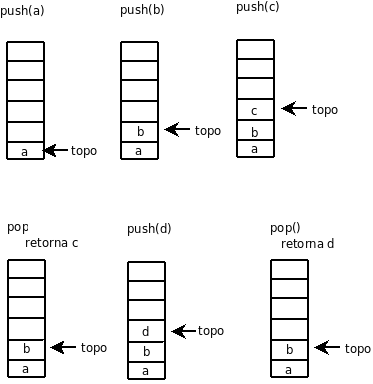
\includegraphics[width=.6\textwidth]{pilha}
			\end{figure} 
   \end{frame}
  
   \begin{frame}{Operações auxiliares}   
			\begin{itemize}
				\item Além das operações básicas, temos as operações ``\textit{auxiliares}''. São elas:
			\end{itemize}
			\begin{table}[ht]
			  \centering
						\begin{tabular}{l|l}
						    \hline \textbf{Operação} & \textbf{Descrição} \\
						    \hline create & cria uma pilha vazia.\\
						    \hline empty(p) & determina se uma pilha \textit{p} está ou não vazia.\\
						    \hline free(p) & libera o espaço ocupado na memória pela pilha \textit{p}.\\
						    \hline 
						\end{tabular}
						\caption{Operações auxiliares da estrutura de dados pilha.}
				\end{table}
  \end{frame}
  
\begin{frame}[fragile,plain]{Interface do Tipo Pilha -- Típica}
\begin{lstlisting}[language=C]
/* Definicao da estrutura */
typedef struct { DEFINA O SEU MODELO AQUI }  Pilha;

/*Aloca dinamicamente ou estaticamente a estrutura pilha, 
  inicializando seus campos e retorna seu ponteiro.*/
Pilha * create(void);

/*Insere o elemento e na pilha p.*/
void push(Pilha *p, int e);

/*Retira e retorna o elemento do topo da pilha p*/
int pop(Pilha *p);

/*Informa se a pilha p esta ou nao vazia.*/
int empty(Pilha *p);
\end{lstlisting}
\end{frame}



\begin{frame}
\frametitle{Implementações} 


\begin{enumerate}

  \item Baseada em um simples vetor
    \item Baseada em um vetor dinâmico
      \item Baseada em lista encadeada
      \pause
      \item mas todas usam ponteiros!


\end{enumerate}


\end{frame}


\begin{frame}{Implementação de Pilha com Vetor}  
	\begin{itemize}
		\item Normalmente as aplicações que precisam de uma 
		estrutura pilha, é comum saber de antemão o número 
		máximo de elementos que precisam estar armazenados 
		simultaneamente na pilha.
		\item Essa estrutura de pilha tem um limite conhecido.
		\item Os elementos são armazenados em um vetor.
		\item Essa implementação é mais simples.
		\item Os elementos inseridos ocupam as primeiras posições do vetor. 
	\end{itemize}
\end{frame}

\begin{frame}{Implementação de Pilha com Vetor}  
	\begin{itemize}
		\item Seja \textit{p} uma pilha armazenada em um vetor \textit{VET} de \textit{N} elementos:		
			\begin{enumerate}
				\item O elemento vet[topo] representa o elemento do topo.
				\item A parte ocupada pela pilha é vet[0 .. topo - 1].
				\item A pilha está vazia se topo = -1.
				\item Cheia se topo = N - 1.
				\item Para desempilhar um elemento da pilha, não vazia,
				 basta $$x = vet[topo--]$$ \textcolor{red}{(recupera valor do topo e depois decrementa)} 
				\item Para empilhar um elemento na pilha, em uma pilha não cheia, 
				basta $$vet[++t] = e$$   \textcolor{red}{(soma antes e depois insere)}
			\end{enumerate}
	\end{itemize}
\end{frame}

\begin{frame}[fragile]{Implementação de Pilha com Vetor}
\begin{lstlisting}[language=C]
#define N 20 /* numero maximo de elementos*/
#include <stdio.h>
#include "pilha.h"

/*Define a estrutura da pilha*/
struct pilha{
  int topo;            /* indica o topo da pilha */
  int elementos[N];   /* elementos da pilha*/
};

Pilha* create(void){
  Pilha* p = (Pilha * ) malloc(sizeof(Pilha));
  p->topo = -1;     /* inicializa a pilha com 0 elementos */
  return p;
}	
	\end{lstlisting}  
\end{frame}

\begin{frame}[fragile,c]{Implementação de Pilha com Vetor}
\begin{itemize}
	\item Empilha um elemento na pilha
\end{itemize}
\begin{lstlisting}[language=C]
void push(Pilha *p, int e){
     if (p->topo == N - 1){ /* capacidade esgotada */
        printf("A pilha esta cheia");
        exit(1);
     }
     /* insere o elemento na proxima posicao livre */
     p->elementos[++p->topo] = e;
}	
\end{lstlisting}  
\end{frame}

%%%
\begin{frame}[fragile,c]{Implementação de Pilha com Vetor}
\begin{itemize}
	\item Desempilha um elemento da pilha
\end{itemize}
\begin{lstlisting}[language=C]
int pop(Pilha *p)
{
     int e;
     if (empty(p)){
        printf("Pilha vazia.\n");
        exit(1);             
     } 
     
     /* retira o elemento do topo */
     e = p->elementos[p->topo--];
     return e;
}	
\end{lstlisting}  
\end{frame}


\begin{frame}[fragile]{Implementação de Pilha com Vetor}
\begin{lstlisting}[language=C]
/**
 * Verifica se a pilha p esta vazia
 */
int empty(Pilha *p)
{
   return (p->t == -1);
}

\end{lstlisting}
\end{frame}

\begin{frame}{Exemplos de Uso}
\begin{itemize}
	\item Na área computacional existem diversas aplicações de pilhas. 
	\item Alguns exemplos são: caminhamento em árvores, chamadas de sub-rotinas por um compilador ou pelo sistema operacional, inversão de uma lista, avaliar expressões, entre outras.
	\item Uma das aplicações clássicas é a conversão e a avaliação de expressões algébricas. Um exemplo, é o funcionamento das calculadoras da HP, que trabalham com expressões pós-fixadas.
\end{itemize}
\end{frame}






%\begin{frame}{Avaliação de Expressões}
%	\begin{itemize}
%		\item Considere as expressões aritméticas abaixo, e imagine que é nosso objetivo avaliar se as expressões estão definidas corretamente.		
%		\begin{enumerate}
%			\item (A + B) / C
%			\item 3 +  \{[2 + (7 * 3)/5] + (C - B)\} 
%		\end{enumerate}
%	\end{itemize}
%\end{frame}
%

\section{Aplicações -- Estudo de Casos}

\begin{frame}[c]{Balanceamento de Parenteses} 

		   	\begin{figure}[!htpb]
				\centering
				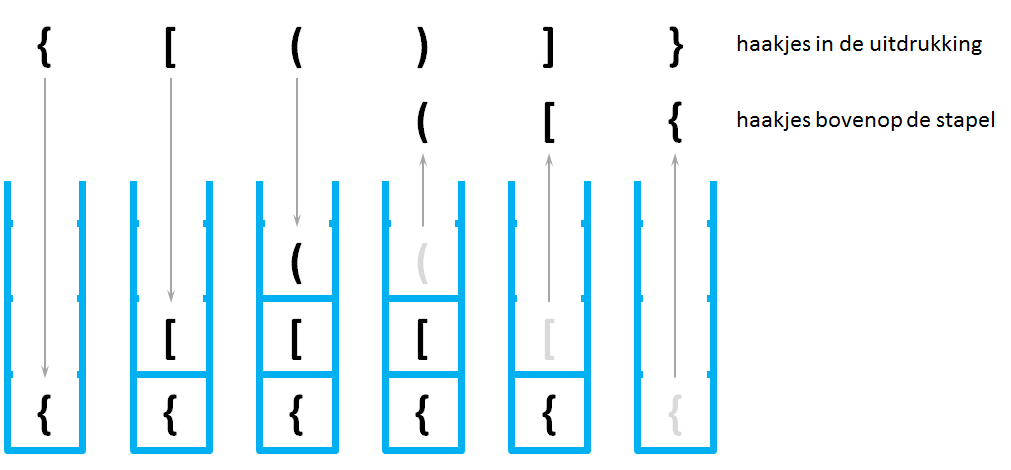
\includegraphics[width=.8\textwidth , height=.7\textheight]{parenteses_balanceado.png}
			\end{figure} 
\end{frame}


\begin{frame}[c]{Balanceamento de Parenteses} 

		\begin{figure}[!htpb]
		\centering
		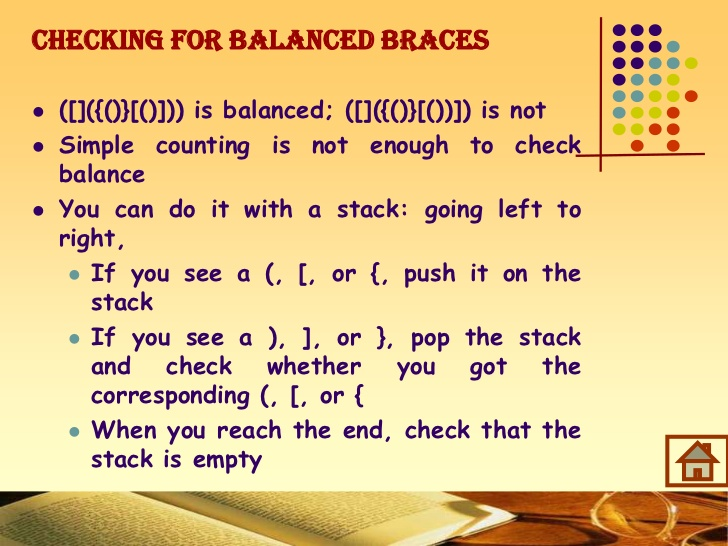
\includegraphics[width=.8\textwidth , height=.7\textheight]{alg_balanceamento.jpg}
		\end{figure} 
\end{frame}


\begin{frame}[c]{Uso imediato: validar expressões Infixas} 

   	\begin{figure}[!htpb]
		\centering
		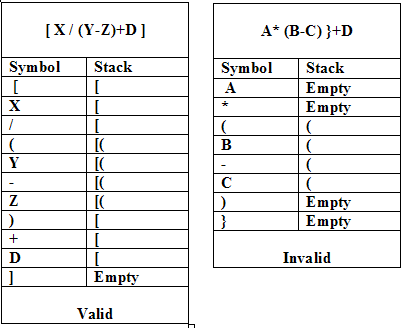
\includegraphics[width=.6\textwidth]{validar_expressoes.png}
		\end{figure} 
\end{frame}



\begin{frame}[c]{Conversão In-fixa para Pós-fixa -- versão 1} 

		   	\begin{figure}[!htpb]
				\centering
				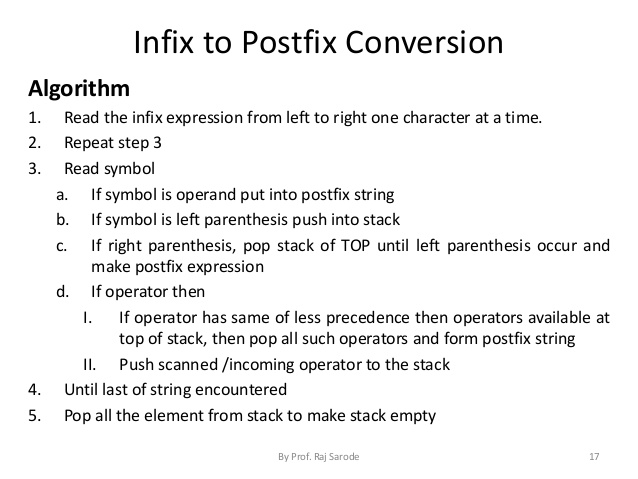
\includegraphics[width=.9\textwidth,height=.8\textheight]{algorit_infix_postfix.jpg}
				\end{figure} 

\end{frame}

\begin{frame}[c]{Conversão In-fixa para Pós-fixa -- versão 2} 

		   	\begin{figure}[!htpb]
				\centering
				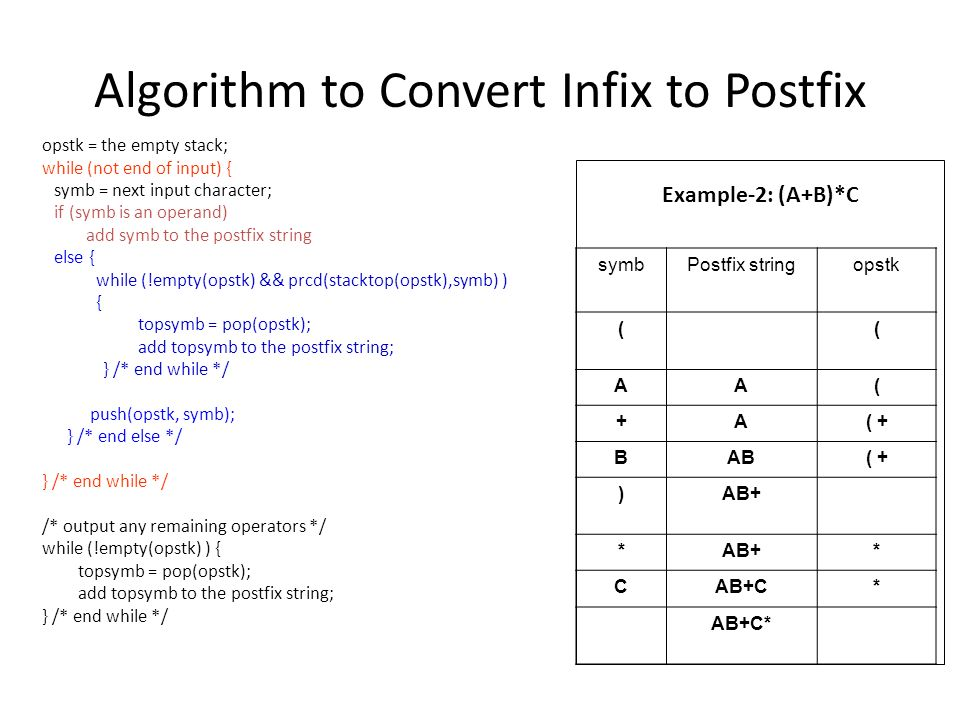
\includegraphics[width=.9\textwidth , height=.8\textheight]{infix_postfix00.jpg}
			\end{figure} 

\end{frame}



\begin{frame}[c]{Conversão In-fixa para Pós-fixa} 

		   	\begin{figure}[!htpb]
				\centering
				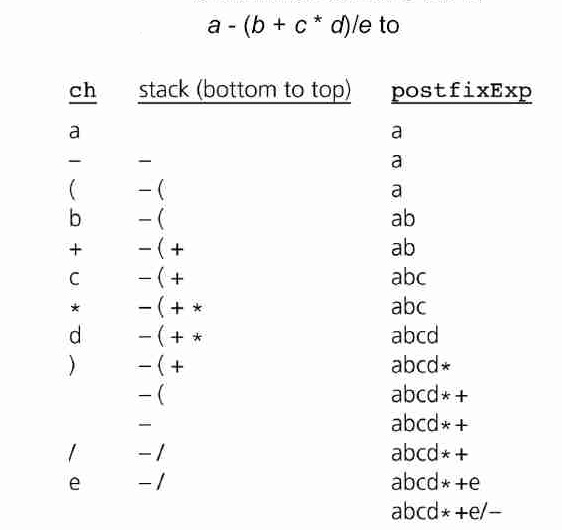
\includegraphics[width=.9\textwidth , height=.8\textheight]{infix_postfix01.jpg}
			\end{figure} 
\end{frame}



\begin{frame}[c]{Uso: cálculo de  expressões pós-fixas (e pré-fixas)} 

		   	\begin{figure}[!htpb]
				\centering
				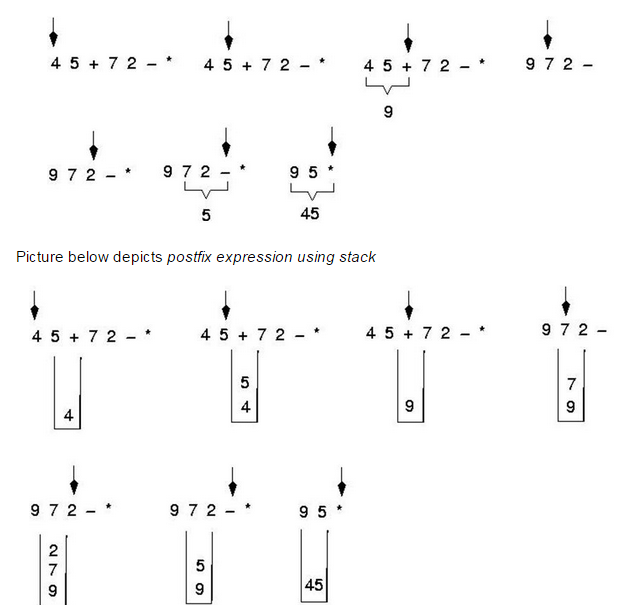
\includegraphics[width=.6\textwidth]{calcula_post_exp.png}
			\end{figure} 
\end{frame}


\begin{frame}[c]{DFS: Busca em Profundidade} 

		   	\begin{figure}[!htpb]
				\centering
				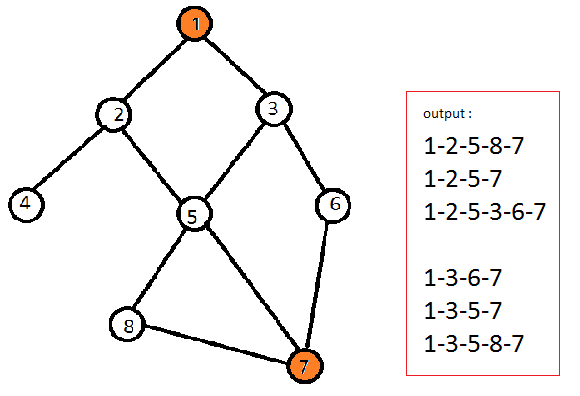
\includegraphics[width=.8\textwidth, height=.7\textheight]{grafo_visitas.png}
			\end{figure} 
\end{frame}



\begin{frame}[c]{DFS: Busca em Profundidade} 

		   	\begin{figure}[!htpb]
				\centering
				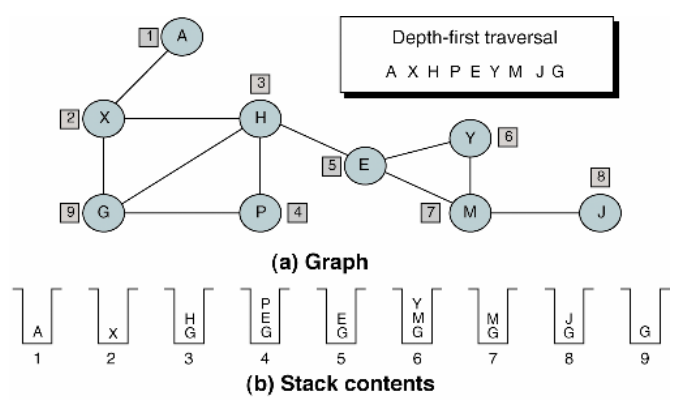
\includegraphics[width=.8\textwidth, height=.7\textheight]{dfs01.png}
			\end{figure} 
\end{frame}



\begin{frame}[c]{DFS: Busca em Profundidade} 

		   	\begin{figure}[!htpb]
				\centering
				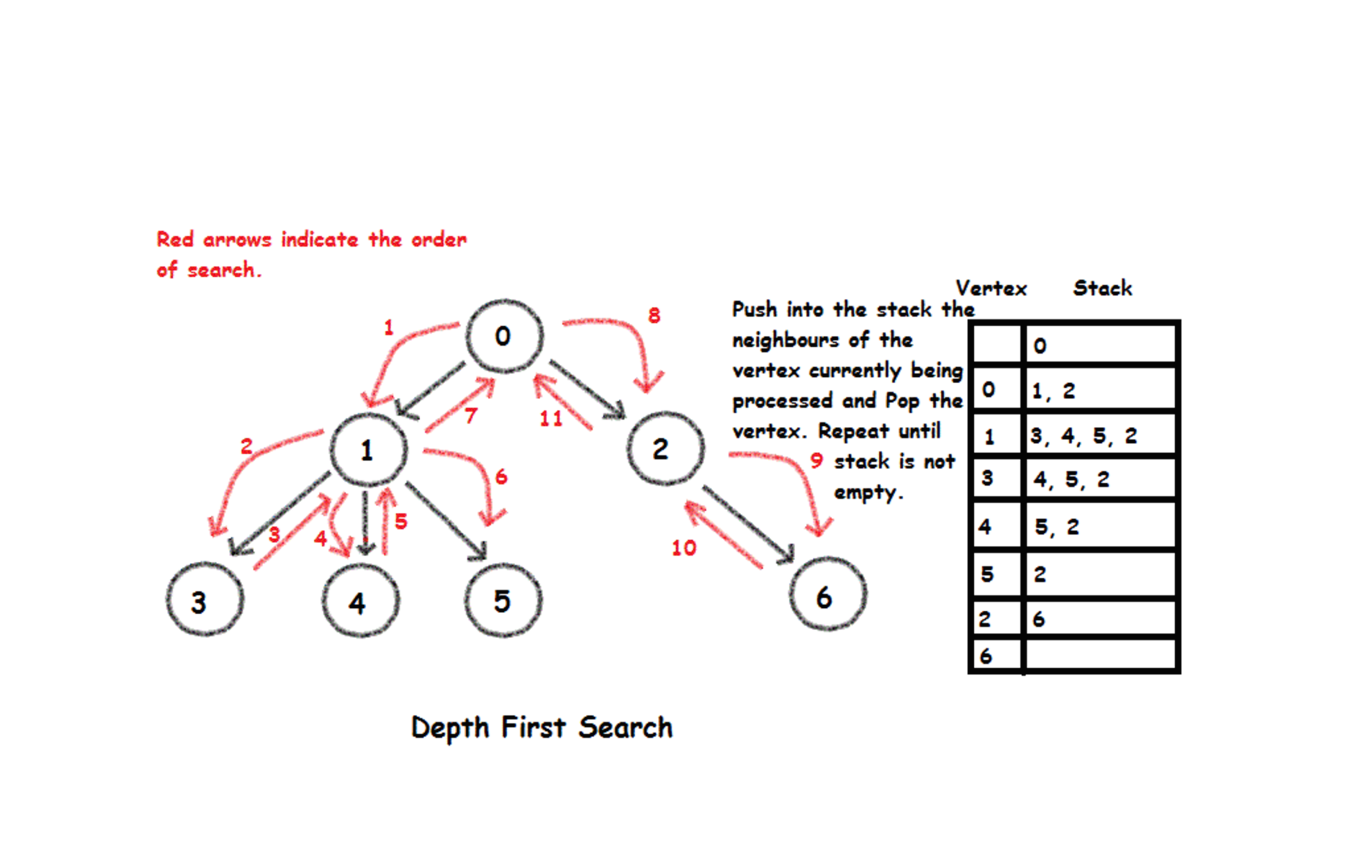
\includegraphics[width=.8\textwidth, height=.7\textheight]{dfs02.png}
			\end{figure} 
\end{frame}


\begin{frame}[c]{Representando Grafos: Matriz de Adjacência} 

		   	\begin{figure}[!htpb]
				\centering
				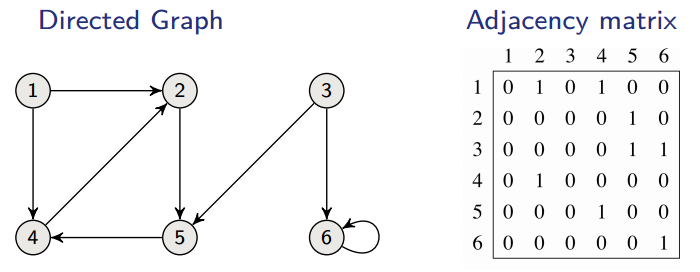
\includegraphics[width=.8\textwidth, height=.5\textheight]{adjacency-matrix.png}
			\end{figure} 
\end{frame}


\begin{frame}[c]{O Algoritmo DFS Iterativo} 

		   	\begin{figure}[!htpb]
				\centering
				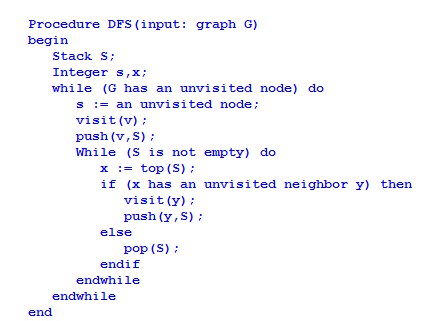
\includegraphics[width=.8\textwidth, height=.7\textheight]{depth-first-search-algorithm01.png}
			\end{figure} 
\end{frame}


\begin{frame}[c]{Ainda sobre o DFS} 

\begin{itemize}
  \item Veloz -- pouca memória
  \item Versátil: muitos tipos de aplicações
  \item Versão recursiva fica ainda mais simples
  \item Evita ciclos com os nós visitados 
  \item Veja a implementação usando pilhas
  
\end{itemize}

\end{frame}



\begin{frame}[fragile]{Exercícios}
	\begin{enumerate}
	
	\item Os exercícios propostos no início deste capítulo (slide inicial)
	
	
		\item Escreva uma função que inverta a ordem das letras de cada palavra de uma sentença, preservando a ordem das palavras. Suponha que as palavras da sentença são separadas por espaços. A aplicação da operação à sentença \textbf{AMU MEGASNEM ATERCES}, por exemplo, deve produzir \textbf{UMA MENSAGEM SECRETA}.
		\item Implemente uma função que receba uma pilha como parâmetro e retorne o valor armazenado em seu topo, restaurando o conteúdo da pilha. Essa função deve obedecer ao protótipo: 
		\begin{verbatim}
		   char topo(Pilha* p);
		\end{verbatim} 
		\item Implemente uma função que receba duas pilhas, $p_1, p_2$, e passe todos os elementos da pilha $p_2$ para o topo da pilha $p_1$. Essa função deve obedecer ao protótipo: 
		\begin{verbatim}
		   void concatena(Pilha* p1, Pilha* p2);
		\end{verbatim} 
	\end{enumerate}
\end{frame}
 % cap 0
%\section{Introdução}
\section{Árvores}

\begin{frame}

\begin{center}
{\Large Capítulo 06 -- Árvores}
\end{center}

Pontos fundamentais a serem cobertos:
\begin{columns}
\begin{column}{.3\textwidth}
\centering

  \begin{enumerate}
  \item Contexto e motivação

  \item Definição

  \item Implementações

  \item Exercícios 

\end{enumerate}  

\end{column}
\begin{column}{.7\textwidth}
\centering
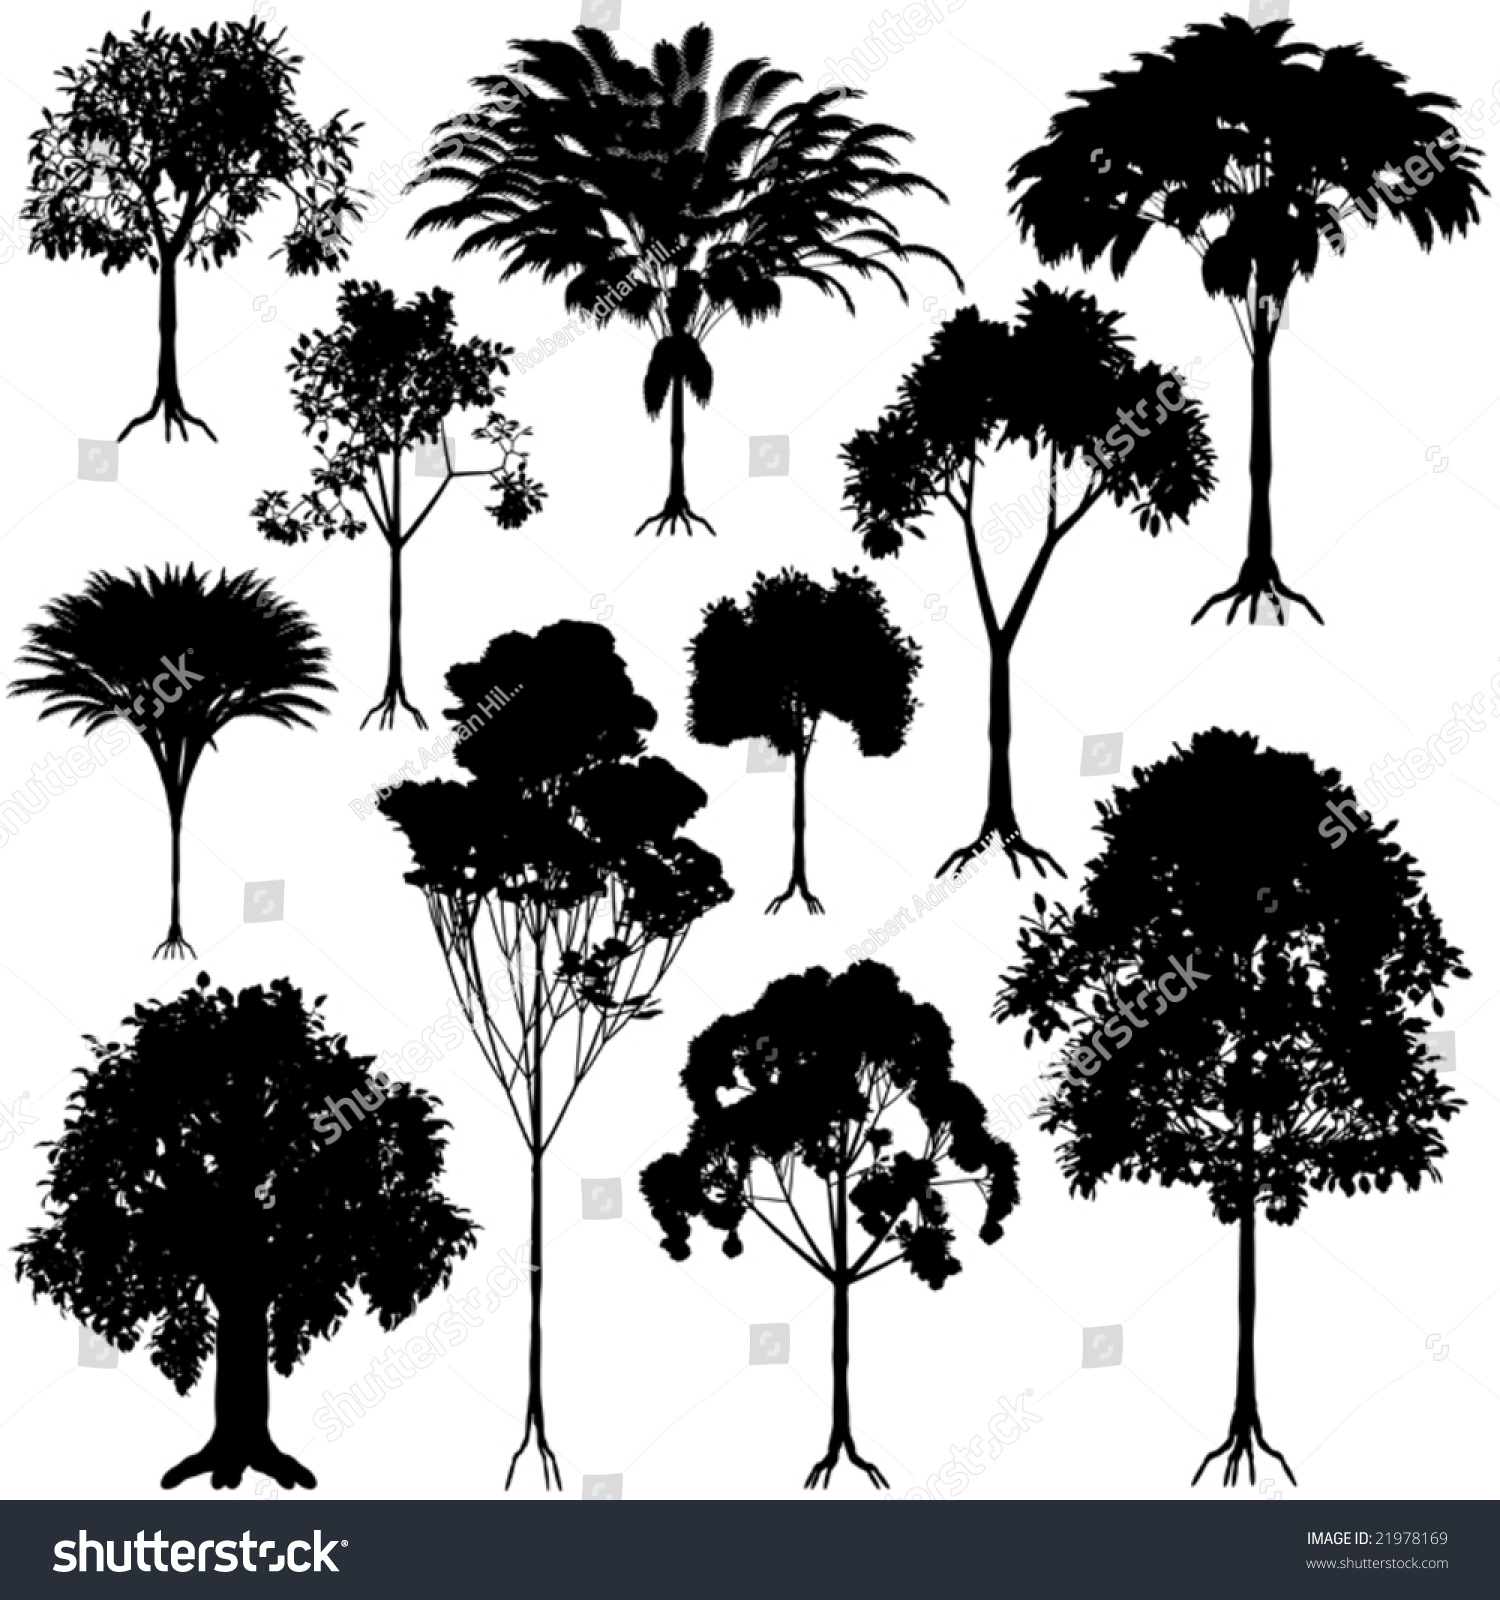
\includegraphics[height=5.3cm, width=7cm]{figs/fig_arvores/arv_CAPA.jpg}
\hspace{+0.25cm}
%\scriptsize\textcolor{red}{[Tizio, Caio et al., Nature (2006)]}
\end{column}
\end{columns}


\end{frame}
%-----------------------------------------------------------------------------
\subsection{Apresentação}

\begin{frame}%[allowframebreaks=0.9, c]

    \frametitle{Definição}
    
    \begin{itemize}
    \item Uma árvore é uma estrutura hierárquica composta por nós e ligações entre eles
    \item Pode ser vista como um grafo acíclico
    \item Cada nó possui somente um pai e zero ou mais filhos
    \item Muitas definições ...
    \end{itemize}
\end{frame}

%---------------------------------------------------------
\begin{frame}%[allowframebreaks=0.9, c]
    \frametitle{Estrutura}
    
    \begin{figure}[tbp]
    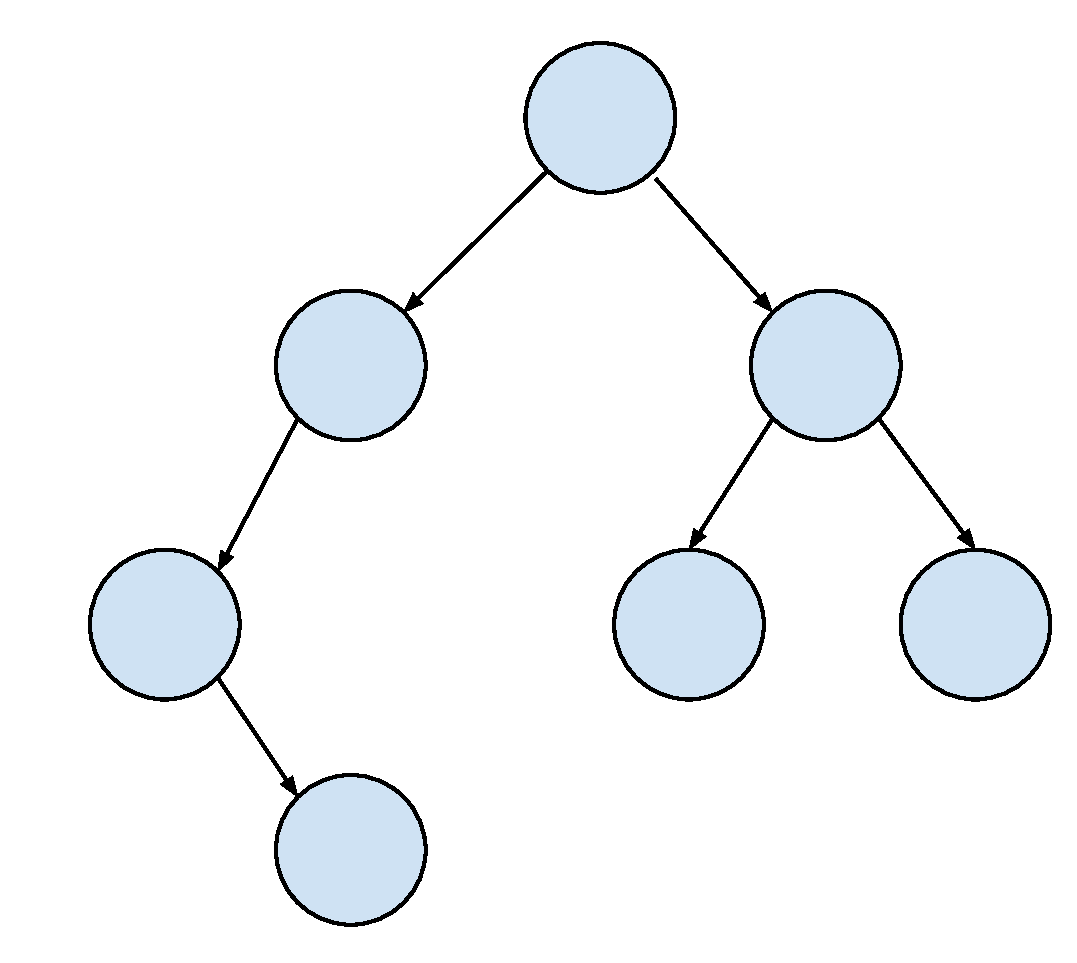
\includegraphics[keepaspectratio=true,width=2.5in]{figs/fig_arvores/arvore.pdf}
    \centering
    \caption{Exemplo de uma árvore}
    \end{figure}
\end{frame}
%---------------------------------------------------------


%---------------------------------------------------------
\begin{frame}
    \frametitle{\textit{Roadmap} para estudo}
    
\begin{block}{mantendo um \textit{foco}:}

\begin{enumerate}
  \item Conceitos de árvores genéricas etc ... 
    \item Árvores Binárias
  \item Árvore Binária de Busca
   \item Árvore AVL (iniciais dos nomes:  \textit{Georgii Adelson-Velsky et Evguenii Landis (en), 
   qui l'ont publié en 1962 sous le titre An Algorithm for the Organization of Information})
   \item Projeto 10\% : 
   \begin{itemize}
     \item  Implemente uma AVL;
    \item   Leia um conjunto de dados numéricos contidos no arquivo fornecido (um valor por linha: string, int, float, char), inserindo-os sequencialmente na AVL implementada;
    \item   Imprima o percurso (valores dos nós) em pré-ordem, em-ordem e pós-ordem, além da altura da árvore
    \item Com a altura dará para ver se a AVL está OK!
   \end{itemize}
  
  \item Vídeos bem legais no Youtube da UNIVEST
  
\end{enumerate}


\end{block}



    \end{frame}

%---------------------------------------------------------
\begin{frame}
    \frametitle{Características -- Requisitos}
    
\begin{itemize}
  
  \item  Como é um nó?
  \item  Qual o grau de um nó?
  \item  Como devem estar estruturados os valores dos nós?
  \item  O que é uma chave do nó?
  \item  O que é a altura?
  \item  Nível?
  \item  Caminhos

\end{itemize}


\end{frame}

%-------------------------------------------------------------------------------------------------------------
\begin{frame}

    \frametitle{Glossário -- 01}
    
     \begin{figure}[!ht]
     \centering
    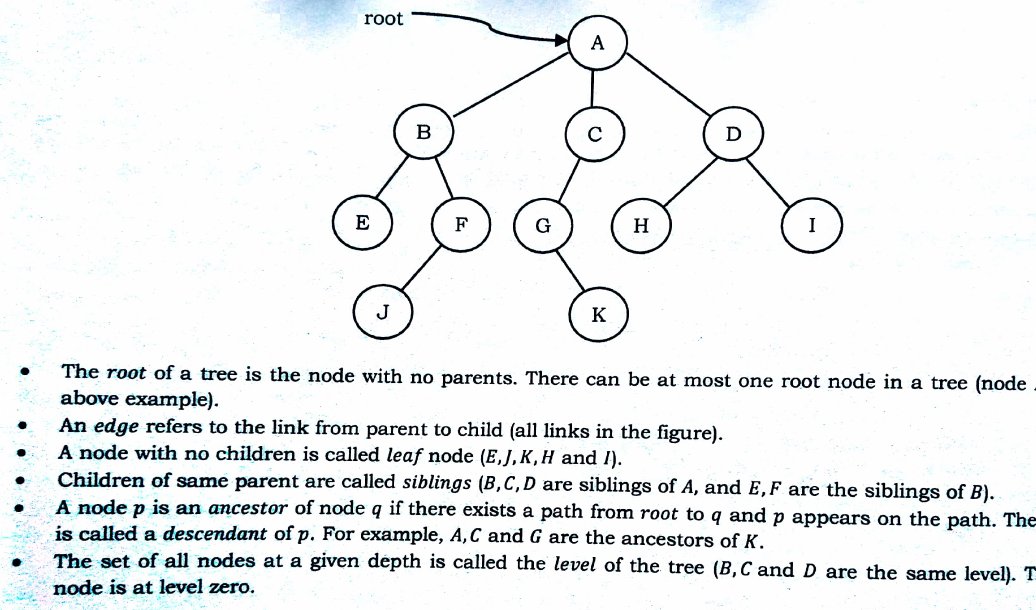
\includegraphics[width=12cm, height=7cm]{figs/fig_arvores/glossario_arv_01.png}
    %\caption{\textcolor{red}{Usando os problemas de árvores genéricas para apresentar Árvores Binárias (AB) }}
    \end{figure}

\end{frame}

%-------------------------------------------------------------------------------------------------------------
\begin{frame}

    \frametitle{Glossário -- 02}
    
     \begin{figure}[!ht]
     \centering
    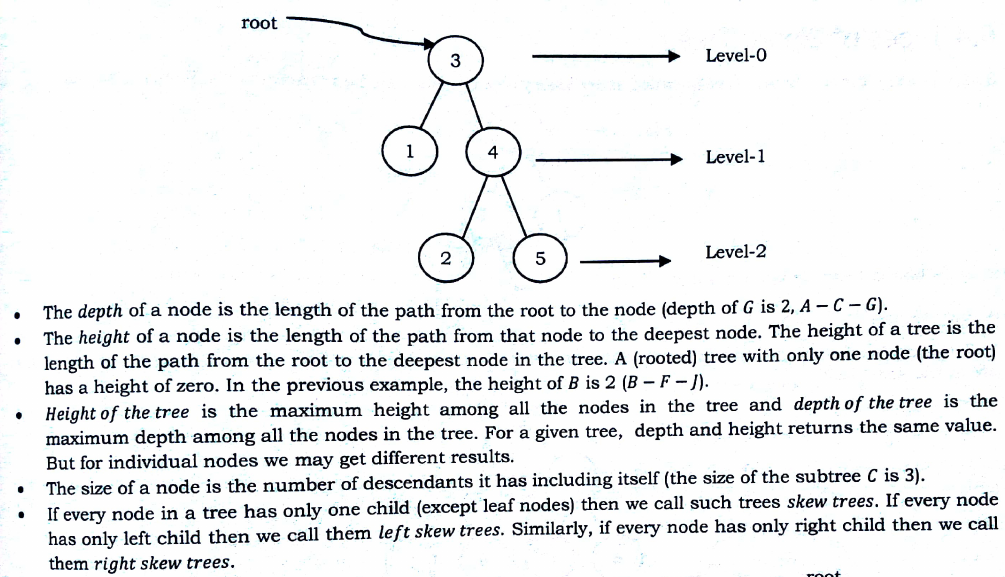
\includegraphics[width=12cm, height=7cm]{figs/fig_arvores/glossario_arv_02.png}
    %\caption{\textcolor{red}{Usando os problemas de árvores genéricas para apresentar Árvores Binárias (AB) }}
    \end{figure}

\end{frame}
%-------------------------------------------------------------------------------------------------------------
\begin{frame}

    \frametitle{Glossário -- 03}
    
     \begin{figure}[!ht]
     \centering
    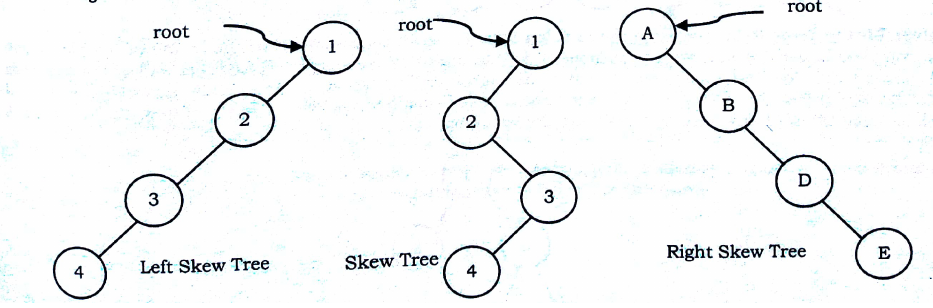
\includegraphics[width=8cm, height=5cm]{figs/fig_arvores/glossario_arv_03.png}
    %\caption{\textcolor{red}{Usando os problemas de árvores genéricas para apresentar Árvores Binárias (AB) }}
    \end{figure}

\end{frame}

%-------------------------------------------------------------------------------------------------------------

\subsection{Árvores Genéricas}

\begin{frame}

    \frametitle{Árvores Genéricas}
    %%Representação  Computacional de 
     \begin{figure}[!ht]
     \centering
    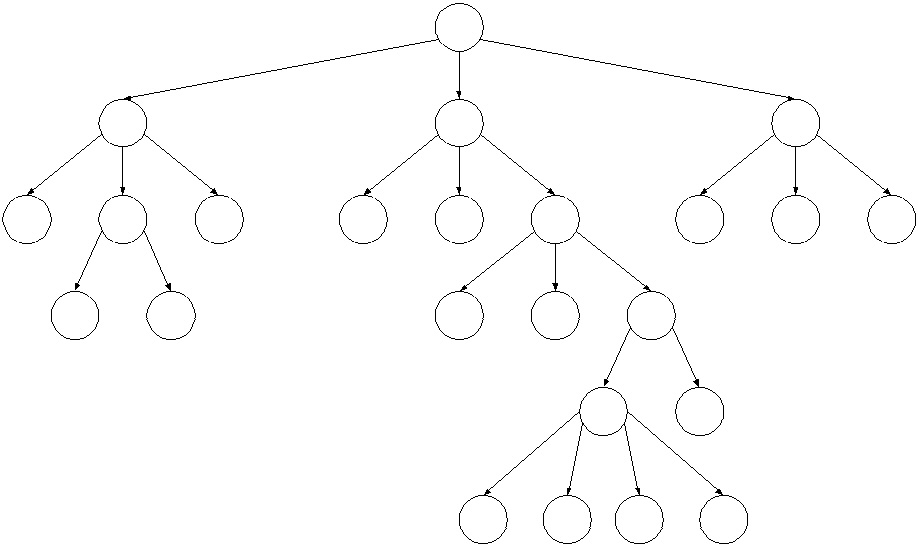
\includegraphics[width=9cm, height=5cm]{figs/fig_arvores/arv_generica01.jpg}
    \caption{\textcolor{red}{Usando os problemas de árvores genéricas para apresentar Árvores Binárias (AB) }}
    \end{figure}

\end{frame}
%-------------------------------------------------------------------------------------------------------------

\begin{frame}

    \frametitle{Transformando uma Árvore Genérica em Binária}
    
     \begin{figure}[!ht]
     \centering
    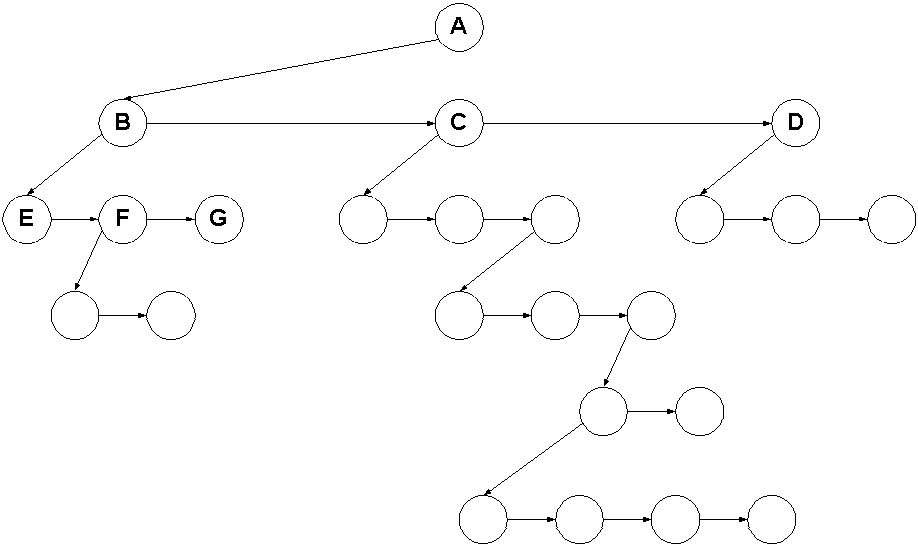
\includegraphics[width=10cm, height=5cm]{figs/fig_arvores/arv_generica02.jpg}
    \caption{\textcolor{red}{Usando os problemas de árvores genéricas para apresentar Árvores Binárias(AB)}}
    \end{figure}

\end{frame}

%-------------------------------------------------------------------------------------------------------------

\begin{frame}

    \frametitle{Representação  Computacional de uma Árvore Genérica}
    
     \begin{figure}[!ht]
     \centering
    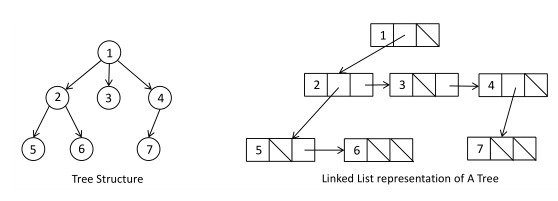
\includegraphics[width=10cm, height=5cm]{figs/fig_arvores/arv_generica03.jpg}
    \caption{\textcolor{red}{Felizmente há um algoritmo que transforme  Árvores Genéricas em Binárias (AB) }}
    \end{figure}

\end{frame}
%-------------------------------------------------------------------------------------------------------------

\begin{frame}

    \frametitle{Representação  Computacional de uma Árvore Genérica}
    
     \begin{figure}[!ht]
     \centering
    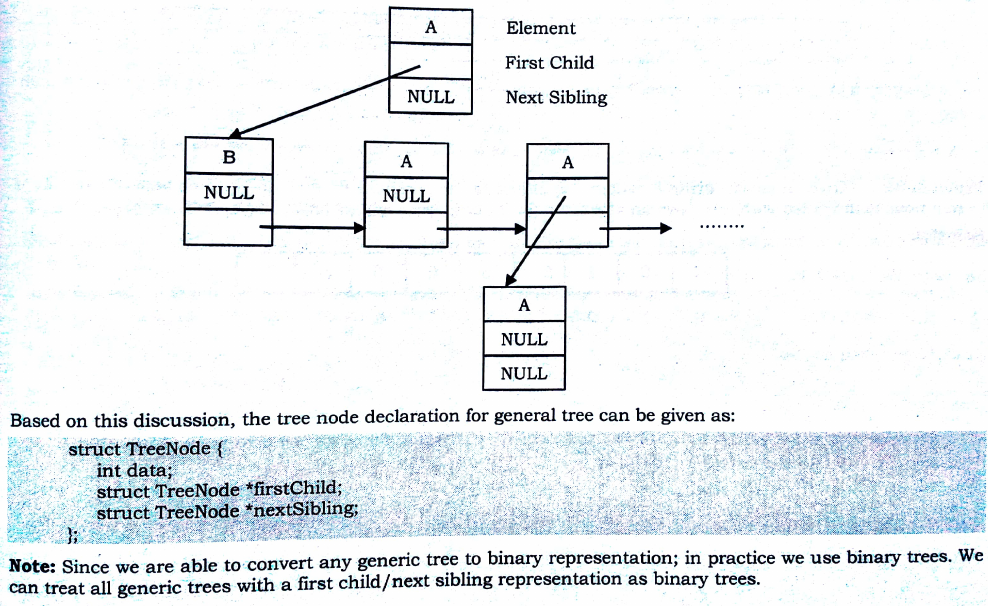
\includegraphics[width=10cm, height=6cm]{figs/fig_arvores/arv_generica04.png}
   \caption{\textcolor{red}{Veja a \textit{struct} ... lembra o quê?}}
    \end{figure}

\end{frame}

%---------------------------------------------------------

\subsection{Aplicações}

\begin{frame}

    \frametitle{Aplicações}

    \begin{itemize}
      \item  Área de compiladores: análise sintática 
      \item  Buscas com complexidade na ordem de: $O(\log n)$ 
     % \item  O uso de Árvores Genéricas foi apenas para motivar as ABBs
      \item  Na área de IA para construção de árvores de decisão: mineração de dados (\textit{big data})
      \item  Organização de taxonomias de conhecimento
      \item  Estruturas hierárquicas em geral      
      
    \end{itemize}    
    
\end{frame}


%---------------------------------------------------------

\begin{frame}

\frametitle{Aplicação  de Árvores}

  \begin{figure}[!ht]
     \centering
    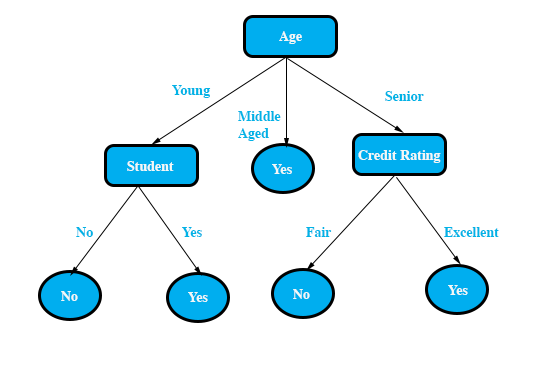
\includegraphics[width=7cm, height=5.5cm]{figs/fig_arvores/aplicacao_decision_tree.png}
    \caption{Árvore de Decisão}
    \end{figure}

\end{frame}

%---------------------------------------------------------

\begin{frame}

    \frametitle{Aplicação  de Árvores}

  \begin{figure}[!ht]
     \centering
    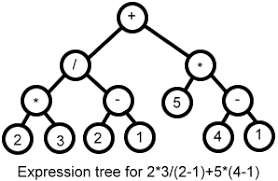
\includegraphics[width=7cm, height=5.5cm]{figs/fig_arvores/aplicacao_expression_tree.png}
    \caption{Árvores de expressões -- binárias -- novamente}
    \end{figure}

\end{frame}

%---------------------------------------------------------

\subsection{Árvore Binária de Busca}

\frame{
    \frametitle{Árvores Binárias de Buscas - ABBs}
    
    
    \begin{itemize}
      \item Árvores Genéricas (AGs): foram utilizadas para motivação as ABBs
      \item Computacionalmente, as ABBs tem um interesse maior que as AGs
      \item Assim, se inicia com ABBs, e seus algoritmos serão adaptados as AGs
    \end{itemize}
    \pause
    
\begin{block}{Definição:}
        
    Árvore onde cada nó possui até 2 filhos. O filho da esquerda só pode conter
    chaves menores do que a do pai, enquanto que o filho da direita só comporta chaves
    maiores do que a do pai.
    \end{block}

}

%---------------------------------------------------------
\frame{
    \frametitle{Árvore Binária de Busca}
    
    \begin{figure}[tbp]
    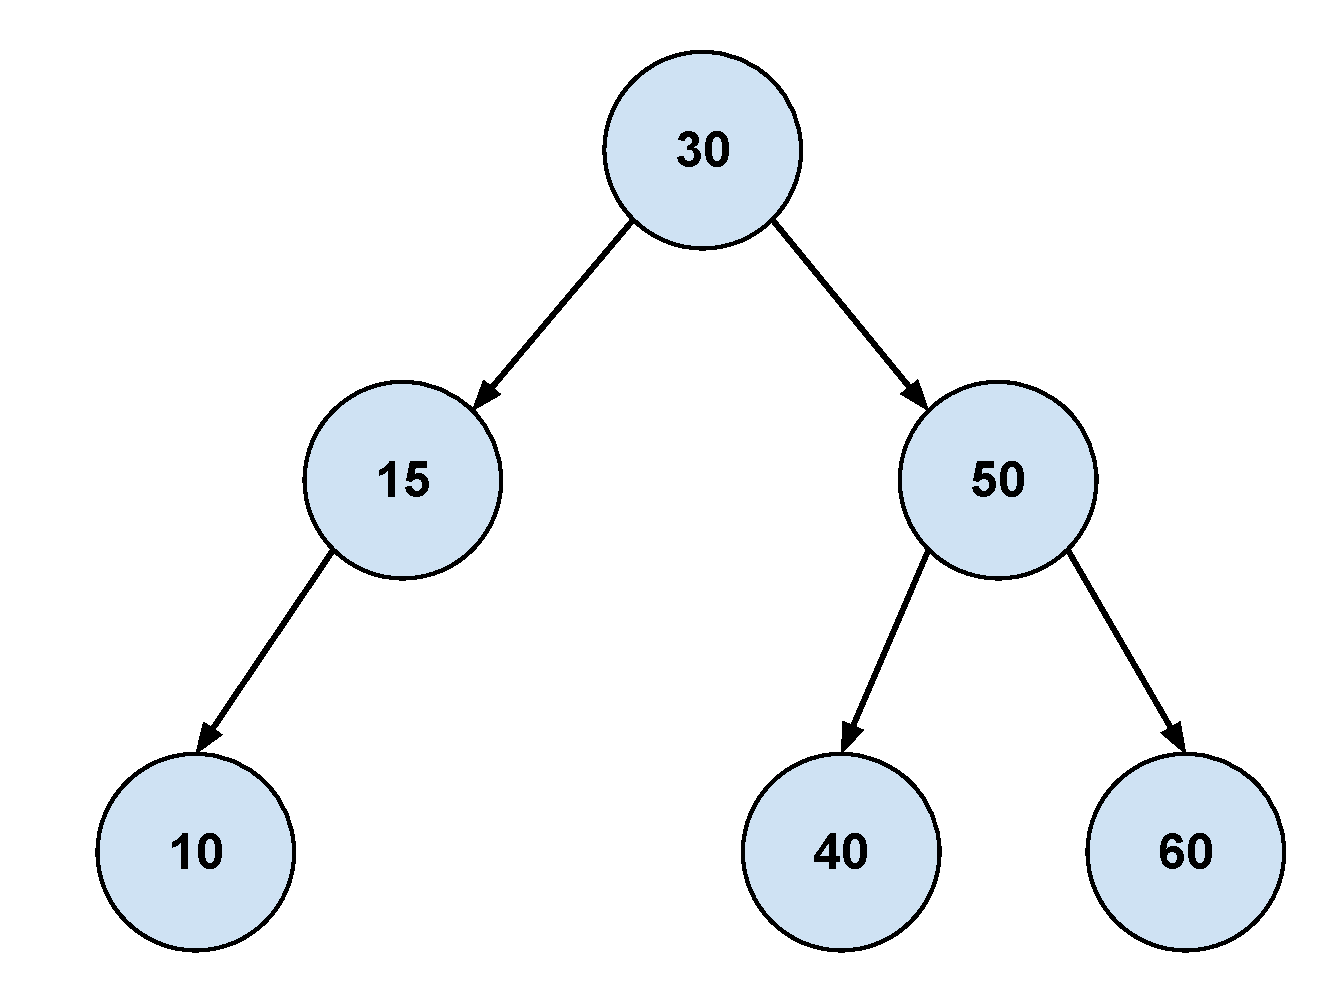
\includegraphics[keepaspectratio=true,width=3in]{figs/fig_arvores/arvore_binaria_de_busca}
    \centering
    \caption{Exemplo de árvore binária de busca}
    \end{figure}
}

%---------------------------------------------------------
\begin{frame}
    \frametitle{Árvore Binária de Busca}
    
    \begin{figure}[tbp]
    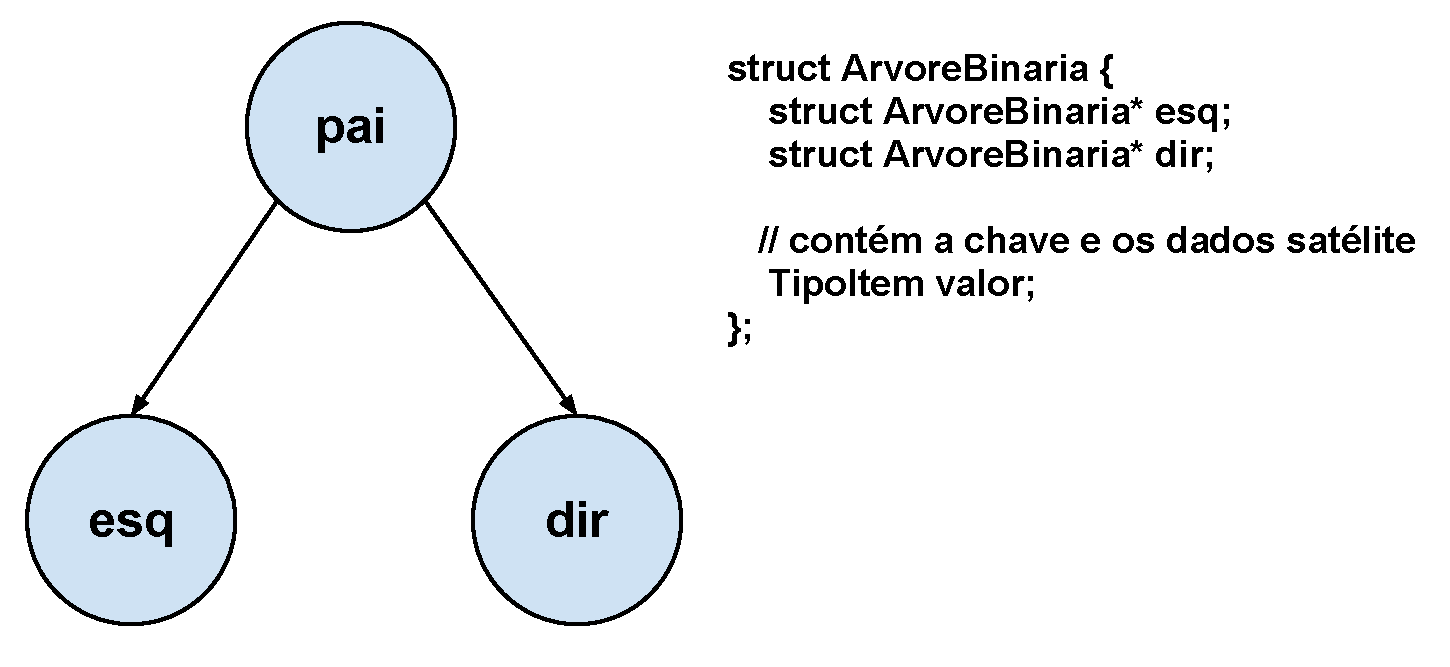
\includegraphics[keepaspectratio=true,width=4in]{figs/fig_arvores/no}
    \centering
    \caption{Estrutura básica / nó}
    \end{figure}

\end{frame}

%---------------------------------------------------------
\frame{
    \frametitle{Operações Básicas}
    
    \begin{block}{Operações Básicas}
    \begin{itemize}
    \item Inserção
    \item Busca
    \item Remoção -- faltando
    \end{itemize}
    \end{block}
    
    \begin{block}{Usos Comuns}
    \begin{itemize}
    \item Dicionários / vetores associativos
    \item Filas de prioridades
    \end{itemize}
    \end{block}
}

%---------------------------------------------------------
\frame{
    \frametitle{Complexidade Computacional}
    
    Quando a árvore está balanceada todas as três operações podem ser implementadas com complexidade
    computacional igual a $O(\log n)$.
    \\ [2em]
    No pior caso (desbalanceamento) estas operações possuem complexidade $O(n)$~\cite{cormen}.
}

%---------------------------------------------------------
\begin{frame}[fragile]
\frametitle{Árvore Binária de Busca - Inserção}
\begin{verbatim}
INSERÇÃO(ARVORE, ITEM) {
    SE ARVORE->CHAVE == NULO
       ARVORE->ITEM = ITEM
       return      //e SE CHAVE jah existente?

    SE ITEM->CHAVE < ARVORE->CHAVE
        SE ARVORE->ESQ = NULO ENTÃO
            ARVORE->ESQ = ARVORE(ITEM)
        SENÃO
            INSERÇÃO(ARVORE->ESQ, ITEM)
    SENÃO
        SE ARVORE->DIR = NULO ENTÃO
            ARVORE->DIR = ARVORE(ITEM)
        SENÃO
            INSERÇÃO(ARVORE->DIR, ITEM)
}
\end{verbatim}
\end{frame}

%---------------------------------------------------------
\frame{
    \frametitle{Árvore Binária de Busca - Inserção}
    
    \begin{figure}[tbp]
    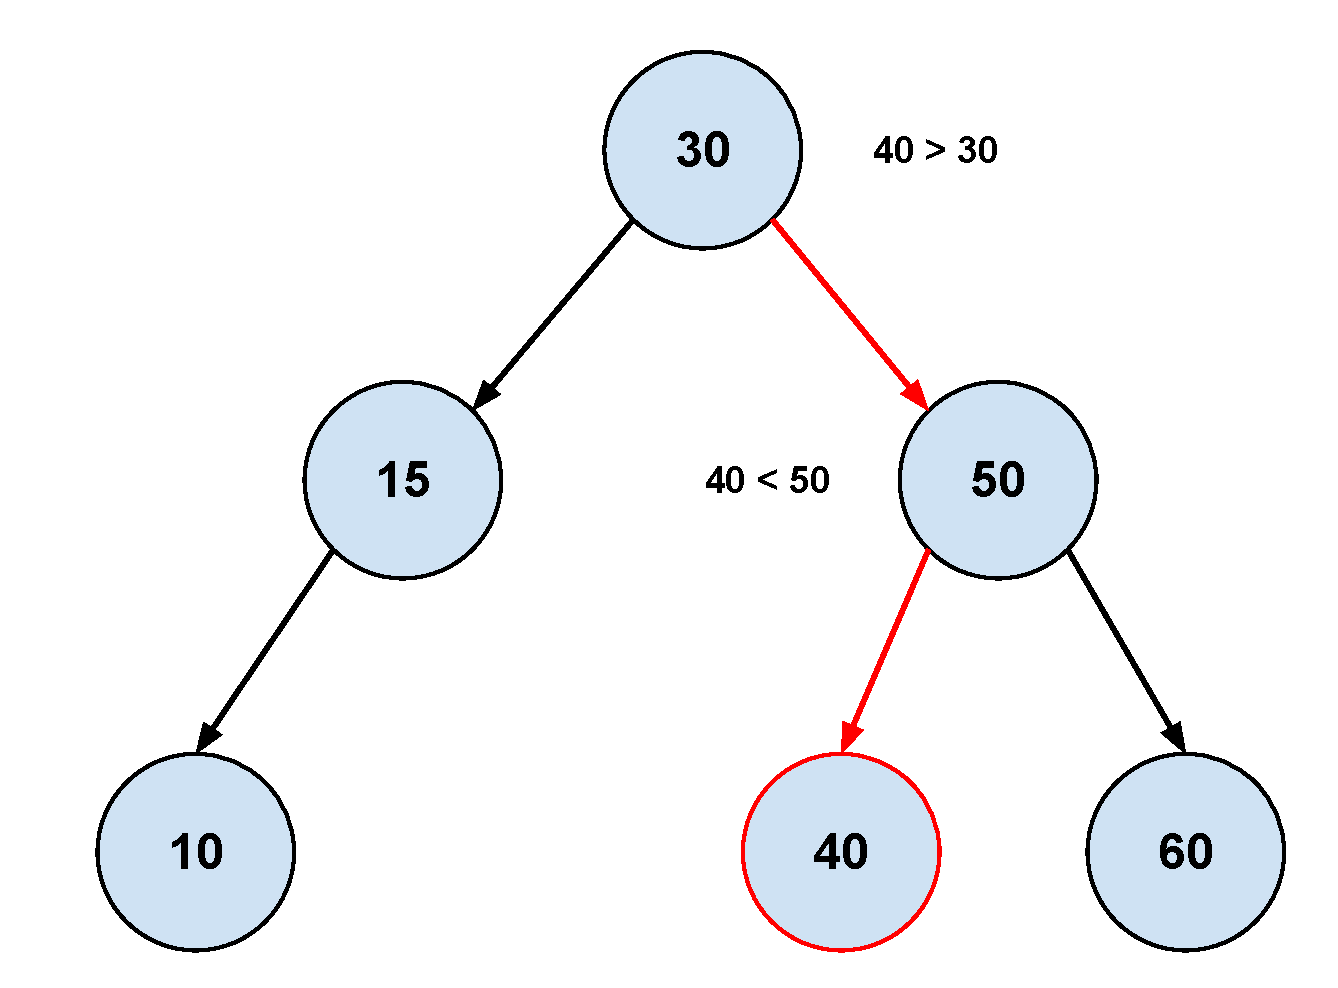
\includegraphics[keepaspectratio=true,width=3in]{figs/fig_arvores/insercao_1}
    \centering
    \caption{Exemplo de inserção da chave 40}
    \end{figure}
}

%---------------------------------------------------------
\frame{
    \frametitle{Árvore Binária de Busca - Inserção}
    
    \begin{figure}[tbp]
    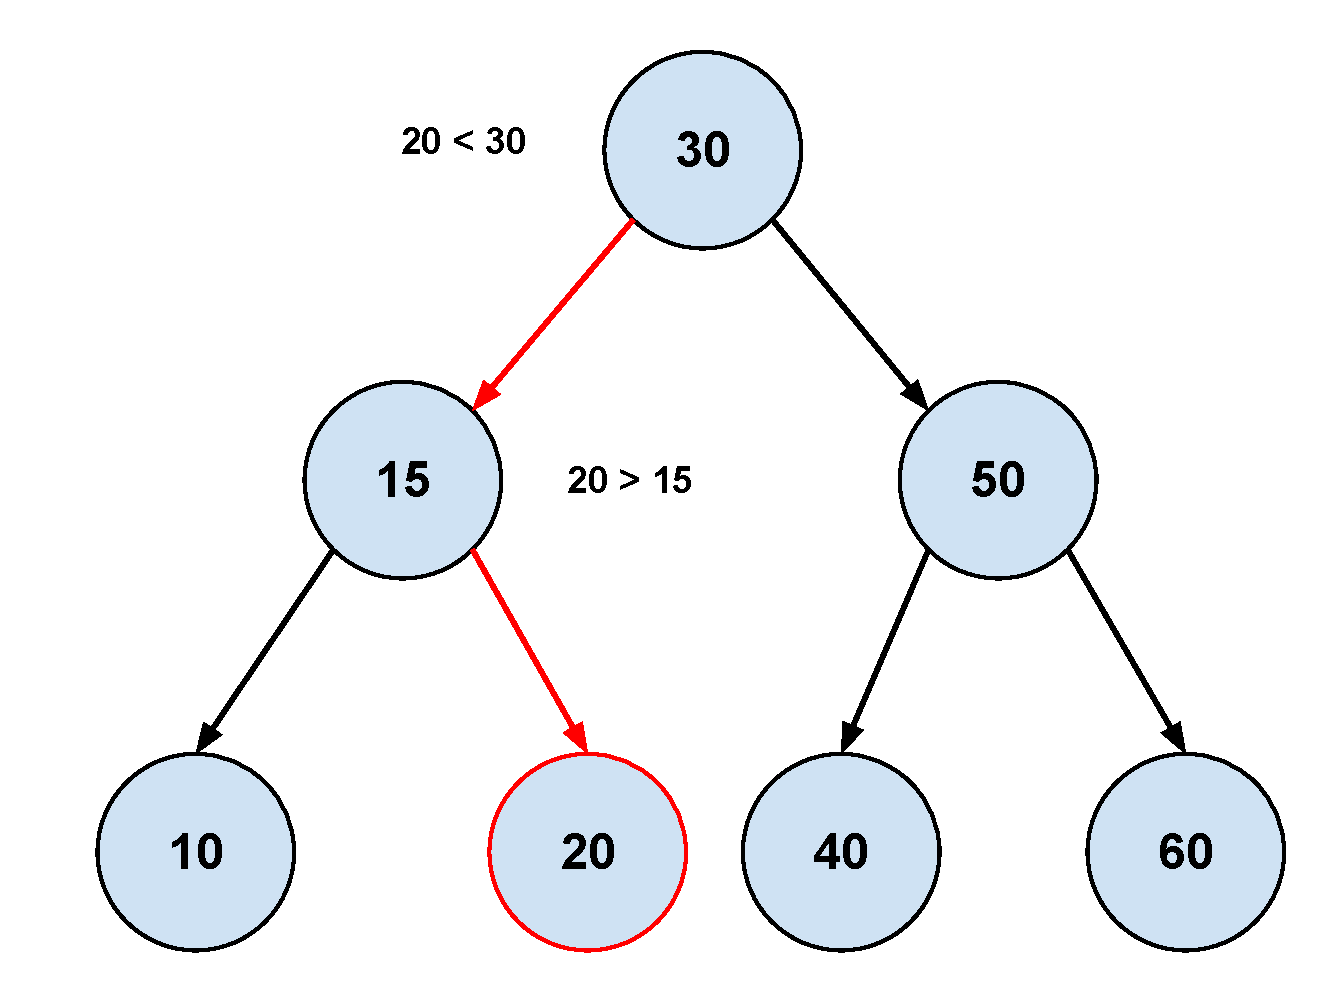
\includegraphics[keepaspectratio=true,width=3in]{figs/fig_arvores/insercao_2}
    \centering
    \caption{Exemplo de inserção da chave 20}
    \end{figure}
}

%---------------------------------------------------------
\begin{frame}[fragile]
\frametitle{Árvore Binária de Busca - Busca}
\begin{verbatim}
BUSCA(ARVORE, CHAVE) {
    SE ARVORE = NULO
        return NULO
        
    SE ARVORE->CHAVE = CHAVE
        return ARVORE
    
    SE CHAVE < ARVORE->CHAVE
        return BUSCA(ARVORE->ESQ, CHAVE)
    SENÃO
        return BUSCA(ARVORE->DIR, CHAVE)
}
\end{verbatim}
\end{frame}

%---------------------------------------------------------
\frame{
    \frametitle{Árvore Binária de Busca -- Remoção}
    
    A remoção de um nó se enquadra em um dos seguintes casos:
    
    \begin{enumerate}
    \item Remoção de um nó folha (nenhum filho)
    \item Remoção de um nó com somente um filho
    \item Remoção de um nó com dois filhos
    \item  \textcolor{red}{Faltam as figuras ainda ....}
    \end{enumerate}

   %% O tratamento de cada caso foi apresentado em sala de aula.
}

%---------------------------------------------------------
\subsection{Balanceamento}

\frame{
    \frametitle{Balanceamento}
    
    Uma árvore binária de busca balanceada garante operações de busca, inserção e
    remoção com complexidade O($\log n$), onde $n$ é o número de nós, o que a torna atrativa
    para diversas aplicações.
    \\[1em]
    Determinadas sequências de inserções ou remoções podem fazer com que uma ABB fique
    desbalanceada, tornando suas operações O($n$).
}

\begin{frame}[fragile]
\frametitle{Cálculo da Altura}
\begin{verbatim}
ALTURA(ARVORE) {
    SE ARVORE = NULO
        return -1
        
    A1 = ALTURA(ARVORE->DIR)
    A2 = ALTURA(ARVORE->ESQ)
    
    return maior(A1, A2) + 1
}
\end{verbatim}
\end{frame}

%---------------------------------------------------------
\begin{frame}
\frametitle{Cálculo da Altura}

\begin{figure}[tbp]
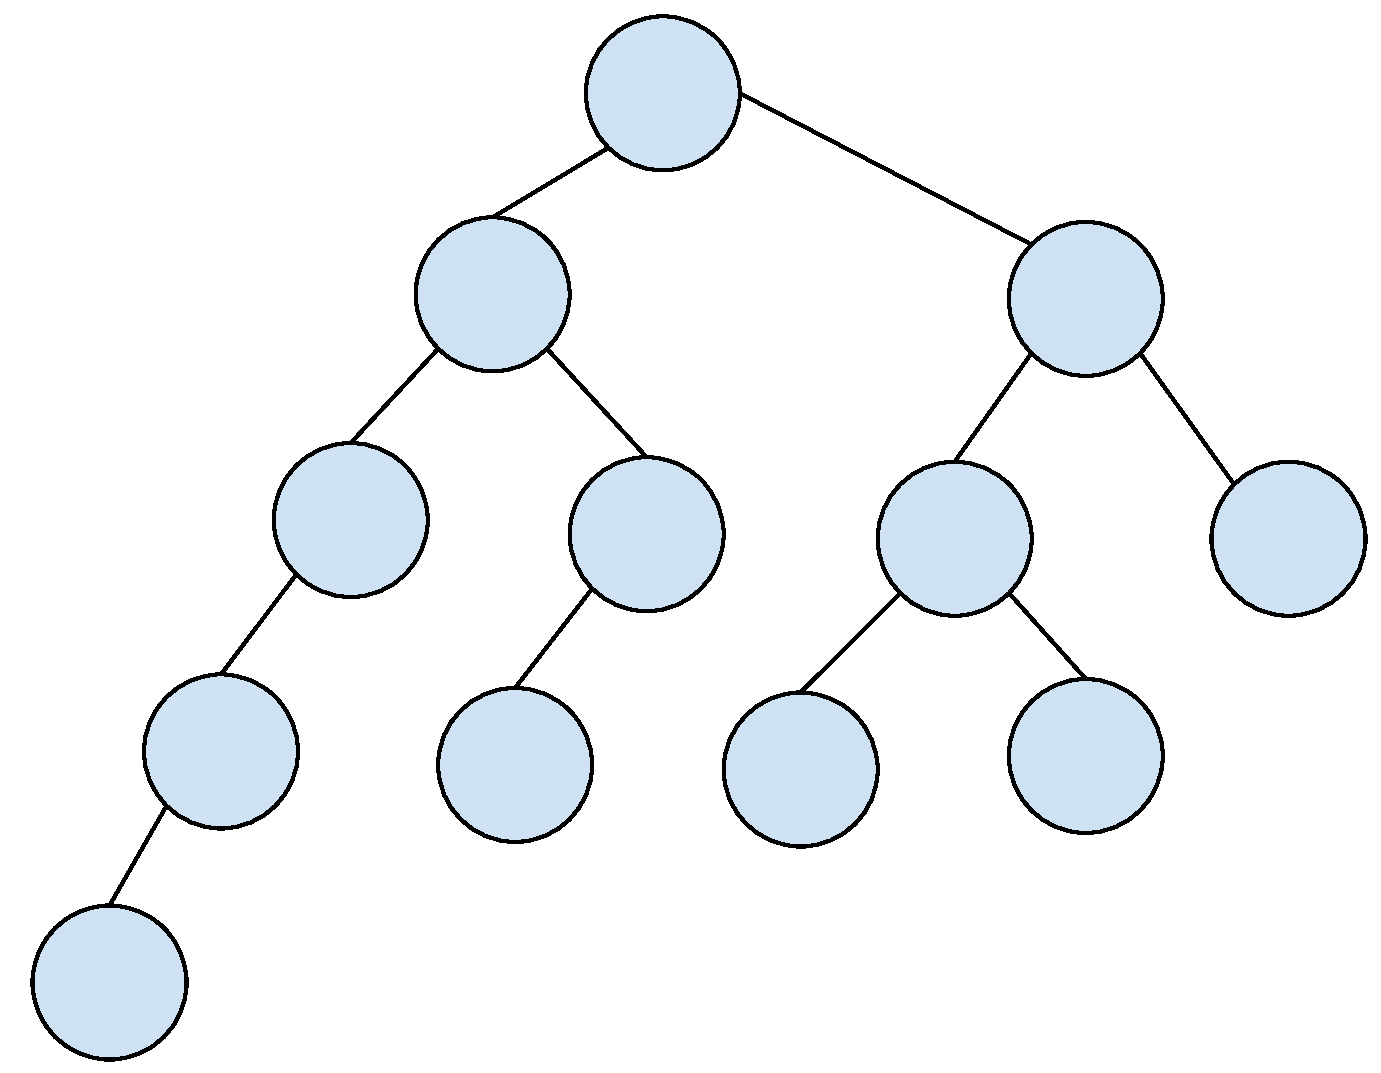
\includegraphics[keepaspectratio=true,width=3in]{figs/fig_arvores/altura1}
\centering
\caption{Exercício: determine a altura de cada subárvore.}
\end{figure}

\end{frame}

%---------------------------------------------------------
\begin{frame}
\frametitle{Cálculo da Altura}

\begin{figure}[tbp]
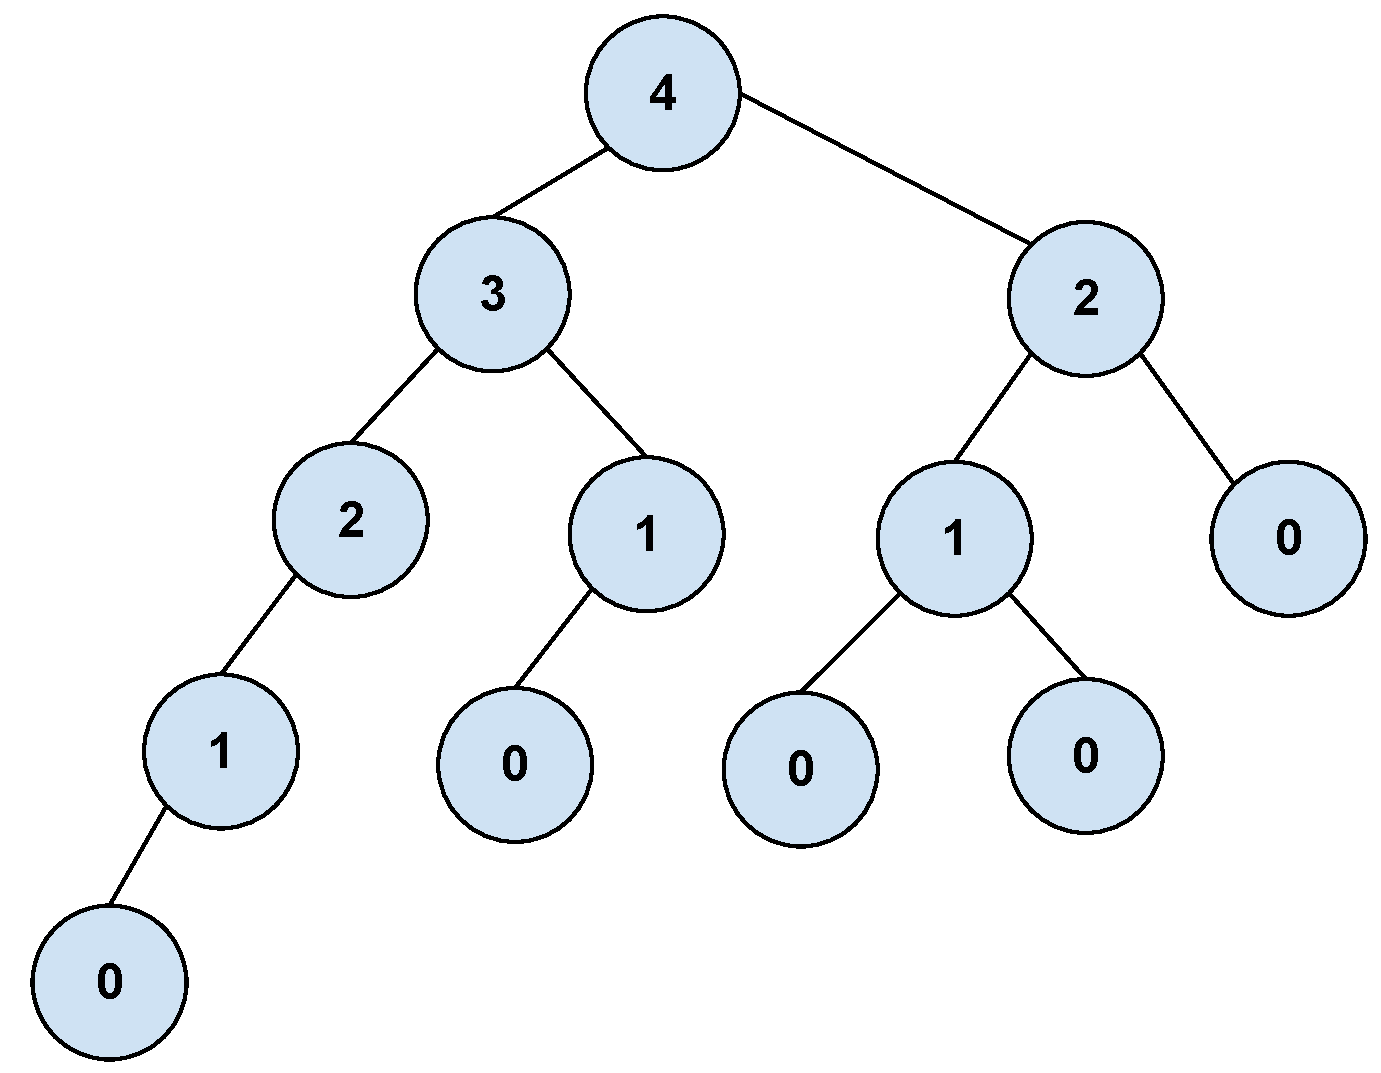
\includegraphics[keepaspectratio=true,width=3in]{figs/fig_arvores/altura2}
\centering
\caption{Resposta do exercício.}
\end{figure}

\end{frame}

%---------------------------------------------------------
\begin{frame}[fragile]
\frametitle{Cálculo do Fator de Balanceamento}
\begin{verbatim}
FB(ARVORE) {
    A1 = ALTURA(ARVORE->ESQ)
    A2 = ALTURA(ARVORE->DIR)
    return A1 - A2 
}
\end{verbatim}
\end{frame}

%---------------------------------------------------------
\frame{
    \frametitle{Balanceamento}
    
    \begin{itemize}
    \item Uma ABB está balanceada quando cada nó possui um FB igual a -1, 0 ou 1
    \item Uma inserção ou remoção pode tornar uma árvore desbalanceada, necessitando de rotações
    para o seu balanceamento
    \end{itemize}
}

%---------------------------------------------------------
\begin{frame}
    \frametitle{Exemplo de ABB Balanceada}
    
    \begin{figure}[tbp]
    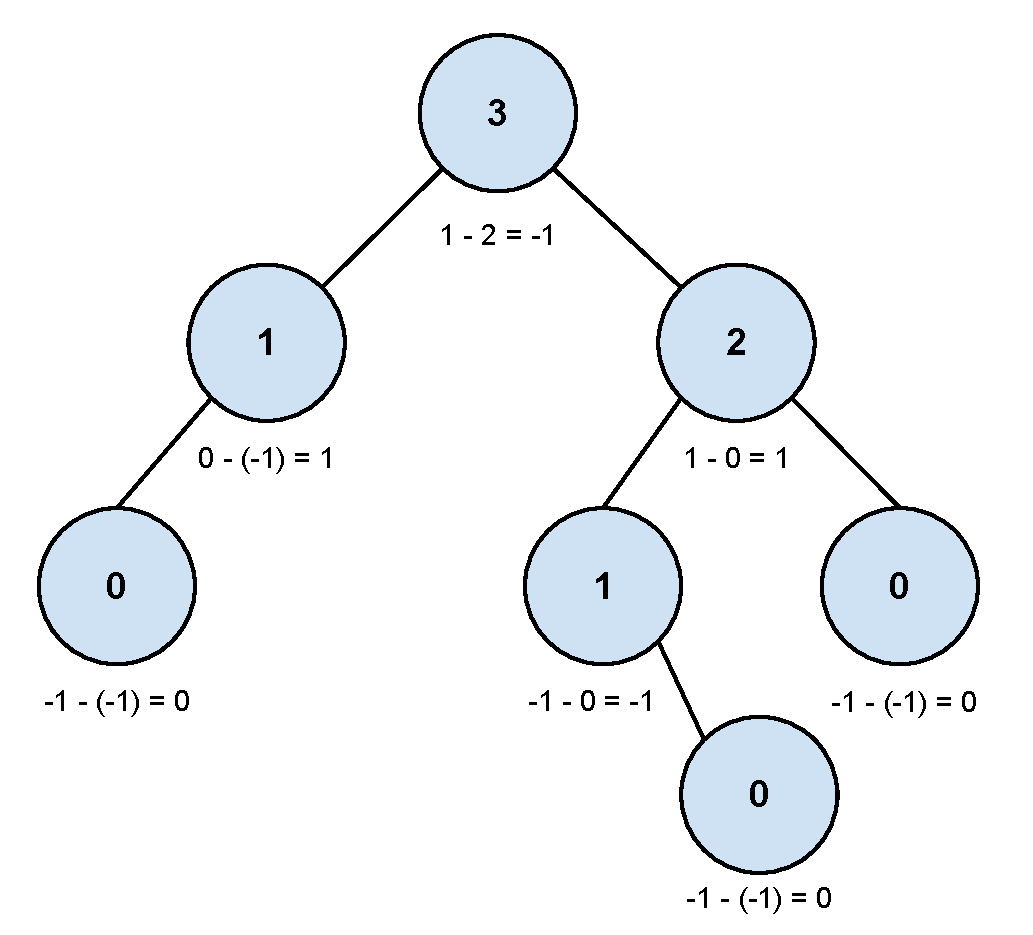
\includegraphics[keepaspectratio=true,width=3in]{figs/fig_arvores/Balanceamento_Arvore}
    \centering
    \end{figure}
\end{frame}

%---------------------------------------------------------
\begin{frame}
    \frametitle{Exemplo de ABB Desbalanceada}
    
    \begin{figure}[tbp]
    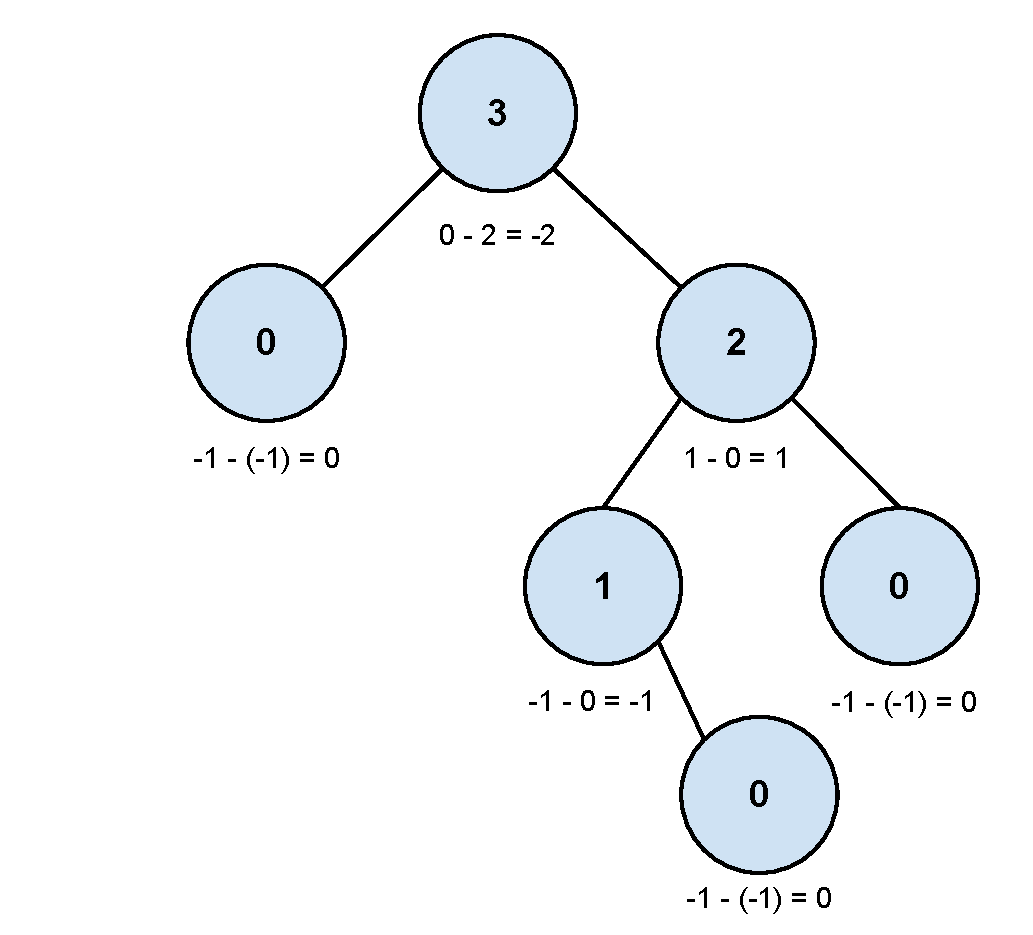
\includegraphics[keepaspectratio=true,width=3in]{figs/fig_arvores/Arvore_Desbalanceada}
    \centering
    \end{figure}
\end{frame}

%---------------------------------------------------------
\subsection{Rotações}

\begin{frame}[fragile]
\frametitle{Operação de rotação}

\begin{verbatim}
ROTACAO_DIREITA(RAIZ) {
    PIVO      = RAIZ->ESQ
    RAIZ->ESQ = PIVO->DIR
    PIVO->DIR = RAIZ
    RAIZ      = PIVO
}
\end{verbatim}

\begin{verbatim}
ROTACAO_ESQUERDA(RAIZ) {
    PIVO      = RAIZ->DIR
    RAIZ->DIR = PIVO->ESQ
    PIVO->ESQ = RAIZ
    RAIZ      = PIVO
}
\end{verbatim}
\end{frame}

%---------------------------------------------------------
\begin{frame}
    \frametitle{Rotação para Direita}
    
    \begin{figure}[tbp]
    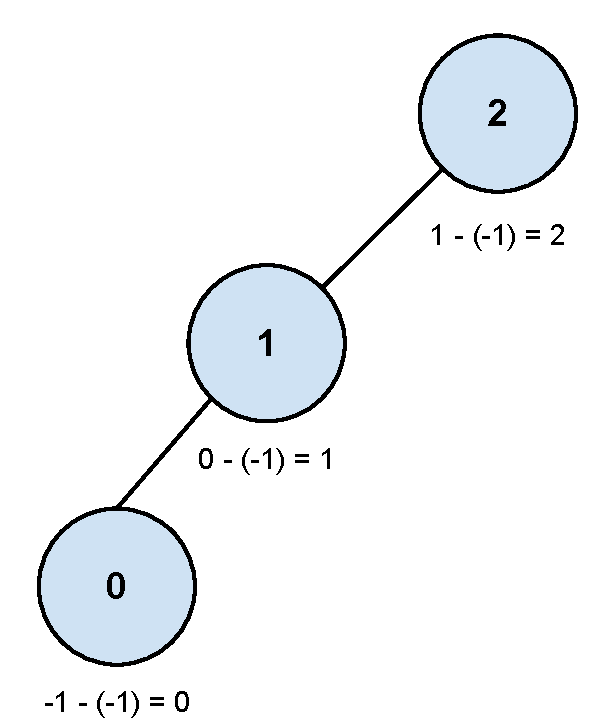
\includegraphics[keepaspectratio=true,width=2.2in]{figs/fig_arvores/Balanceamento_Arvore2}
    \centering
    \end{figure}
\end{frame}

%---------------------------------------------------------
\begin{frame}
    \frametitle{Rotação para Direita}
    
    \begin{figure}[tbp]
    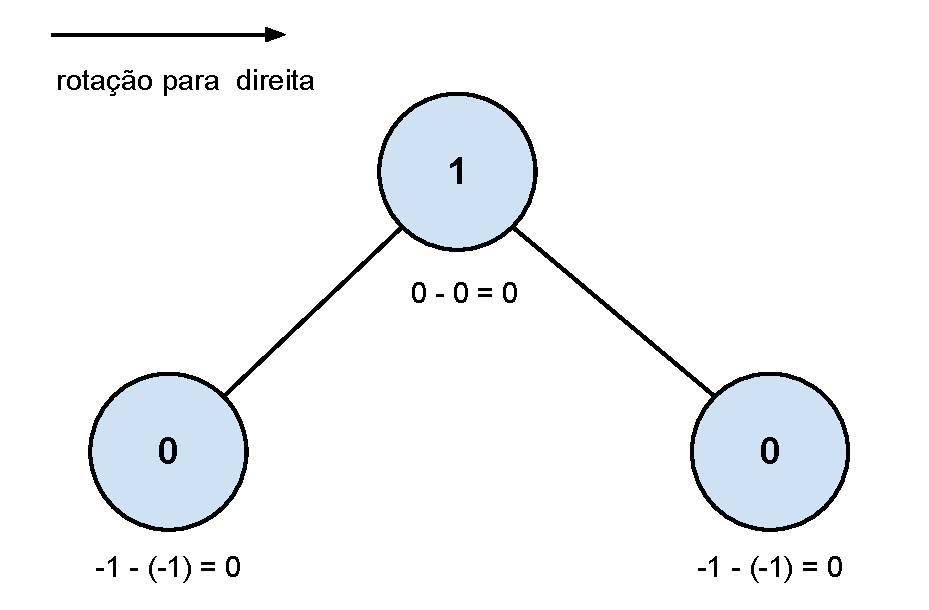
\includegraphics[keepaspectratio=true,width=3.5in]{figs/fig_arvores/Balanceamento_Arvore3}
    \centering
    \end{figure}
\end{frame}


%---------------------------------------------------------
\begin{frame}
    \frametitle{Rotação para Esquerda}
    
    \begin{figure}[tbp]
    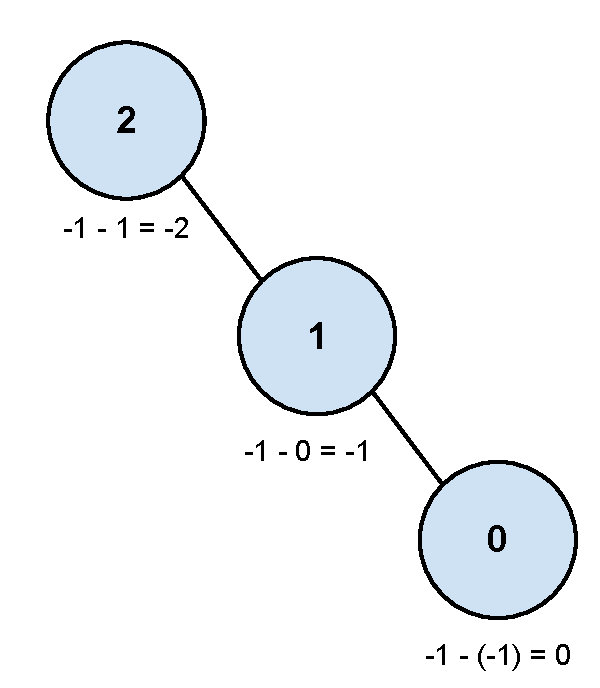
\includegraphics[keepaspectratio=true,width=2.2in]{figs/fig_arvores/Balanceamento_Arvore4}
    \centering
    \end{figure}
\end{frame}

%---------------------------------------------------------
\begin{frame}
    \frametitle{Rotação para Esquerda}
    
    \begin{figure}[tbp]
    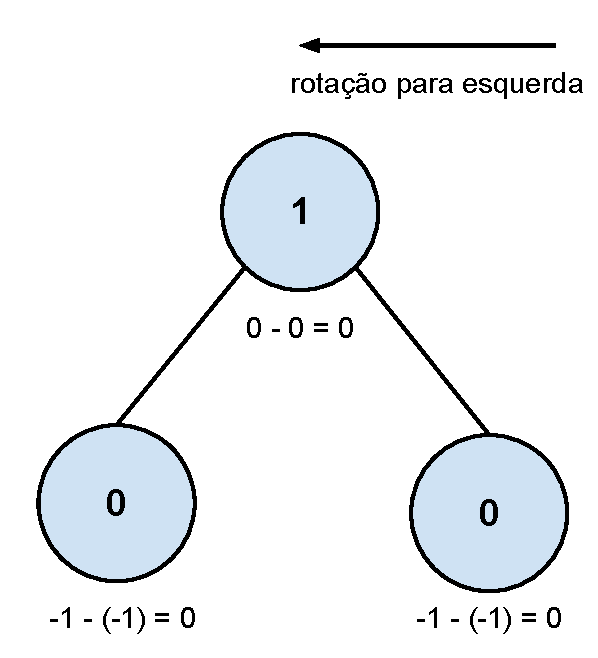
\includegraphics[keepaspectratio=true,width=2.2in]{figs/fig_arvores/Balanceamento_Arvore5}
    \centering
    \end{figure}
\end{frame}

%---------------------------------------------------------
\subsection{Árvores AVL}

\begin{frame}
    \frametitle{Árvores AVL}
    
    \begin{itemize}
    \item \textbf{AVL} desenvolvida por G. M. \textbf{A}delson-\textbf{V}elskii and E. M. \textbf{L}andis
    \item Garante o balanceamento da árvore ao realizar rotações após cada inserção ou remoção na ABB
    \end{itemize}
\end{frame}

%---------------------------------------------------------
\begin{frame}[fragile]
\frametitle{Balanceamento - Inserção}
\begin{verbatim}
BALANCEAMENTO(RAIZ) {
    SE FB(RAIZ) = -2 ENTÃO
        SE FB(RAIZ->DIR) = -1 ENTÃO
            ROTACAO_ESQUERDA(RAIZ)
        SENÃO
            ROTACAO_DIREITA(RAIZ->DIR)
            ROTACAO_ESQUERDA(RAIZ)
    SENÃO SE FB(RAIZ) = 2 ENTÃO
        SE FB(RAIZ->ESQ) = 1 ENTÃO
            ROTACAO_DIREITA(RAIZ)
        SENÃO
            ROTACAO_ESQUERDA(RAIZ->DIR)
            ROTACAO_DIREITA(RAIZ)
}
\end{verbatim}
\end{frame}

%---------------------------------------------------------
\begin{frame}[fragile]
\frametitle{Balanceamento - Inserção}

\begin{itemize}
\item Para que a árvore tenha um bom desempenho, é essencial que o balanceamento seja
calculado eficientemente, isto é, sem a necessidade de percorrer toda a árvore após cada
modificação
\item Manter a árvore estritamente balanceada após cada modificação tem seu preço (desempenho).
Árvores AVL são utilizadas normalmente onde o número de consultas é muito maior do que o número de inserções
e remoções e quando a localidade de informação não é importante
\end{itemize}
\end{frame}

%---------------------------------------------------------
\subsection{Árvore de Espalhamento}

\frame{
    \frametitle{Árvore de Espalhamento}
    
    \begin{itemize}
    \item Reestrutura a árvore em cada operação de inserção, busca ou remoção por meio de operações de rotação
    \item Nome original: \emph{splay tree}~\cite{tarjan}. Não confundir com a Árvore N-Ária de Espalhamento (ANE) criada por professores da UDESC
    \end{itemize}
}

%---------------------------------------------------------
\frame{
    \frametitle{Árvore de Espalhamento}
    
    \begin{itemize}
    \item Evita a repetição de casos ruins [O(n)] devido ao seu rebalanceamento natural
    \item Não realiza o cálculo de fatores de balanceamento, simplificando sua implementação
    \item Pior caso para uma operação se mantém O(n), mas, ao considerar uma cadeia de operações,
    \emph{garante} uma complexidade amortizada de O($\log$n) para suas operações básicas
    \end{itemize}
}

%---------------------------------------------------------
\frame{
    \frametitle{Árvore de Espalhamento}
    
    \begin{itemize}
    \item Se baseia na operação de espalhamento, que utiliza rotações para mover uma determinada
    chave até a raiz
    \item A sua complexidade O($\log$ n) em uma análise amortizada é garantida pelas rotações efetuadas, o que
    a difere do uso simples de heurísticas como o \emph{mover para a raíz}
    \end{itemize}
}

%---------------------------------------------------------
\frame{
    \frametitle{Exemplo - Espalhamento pela chave 1}
    
    \begin{figure}[tbp]
    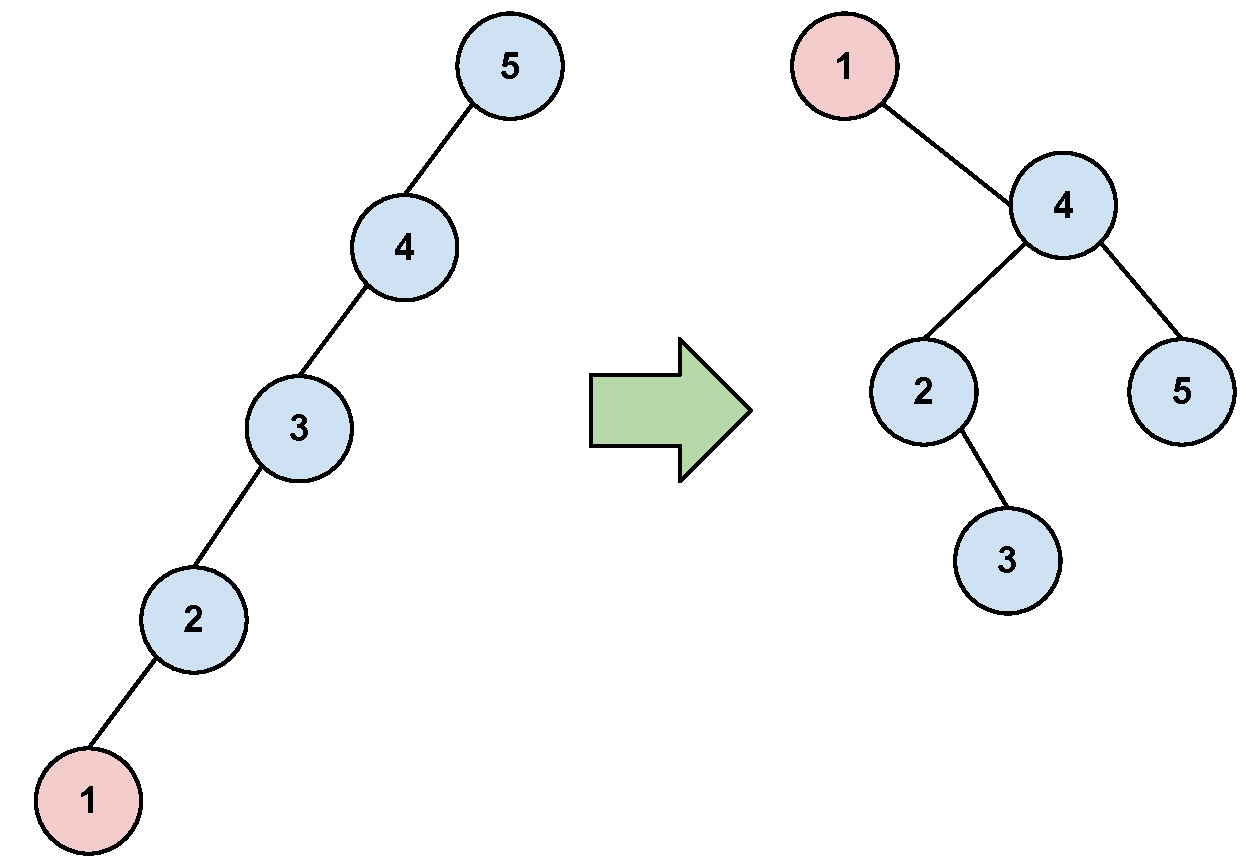
\includegraphics[keepaspectratio=true,width=3.5in]{figs/fig_arvores/Espalhamento}
    \centering
    \end{figure}
}

%---------------------------------------------------------
\frame{
    \frametitle{Operações Básicas}
    
    \begin{description}
    \item[Espalhamento] Move a chave desejada para a raiz por uma
    sequência bem definida de operações de rotação
    \item[Busca] Busca uma chave na árvore
    \item[Inserção] Insere uma nova chave na árvore
    \item[Remoção] Remove uma chave da árvore
    \end{description}
}

%---------------------------------------------------------
\frame{
    \frametitle{Operações Básicas}
    
    \begin{itemize}
    \item Uma árvore de espalhamento é uma árvore binária de busca válida,
    logo operações como os percursos (pré-em-pós) são idênticas as operações
    em uma ABB
    \item As operações de inserção, busca e remoção podem ser definidas com base
    na operação de espalhamento
    \end{itemize}
}

%---------------------------------------------------------
\begin{frame}[fragile]
\frametitle{Árvore de Espalhamento - Busca}
\begin{verbatim}
BUSCA(RAIZ, CHAVE) {
    return ESPALHAMENTO(RAIZ, CHAVE)
}
\end{verbatim}
\end{frame}

%---------------------------------------------------------
\begin{frame}[fragile]
\frametitle{Árvore de Espalhamento - Inserção}
\begin{verbatim}
INSERE(RAIZ, CHAVE) {
    INSERE_ABB(RAIZ, CHAVE)
    return ESPALHAMENTO(RAIZ, CHAVE)
}
\end{verbatim}
\end{frame}

%---------------------------------------------------------
\begin{frame}[fragile]
\frametitle{Árvore de Espalhamento - Remoção}
\begin{verbatim}
REMOVE(RAIZ, CHAVE) {
    RAIZ = ESPALHAMENTO(RAIZ, CHAVE)
    
    SE RAIZ->DIR ENTÃO
        AUX = ESPALHAMENTO(RAIZ->DIR, CHAVE)
        AUX->ESQ = RAIZ->ESQ
    SENÃO
        AUX = RAIZ->ESQ
    
    return AUX
}
\end{verbatim}
\end{frame}

%---------------------------------------------------------
\frame{
    \frametitle{Estratégias de Espalhamento}
    
    Duas estratégias:
    
    \begin{description}
    \item[Bottom-Up] Parte do nó acessado e o movimenta para a raiz da árvore por meio de rotações
    \item[Top-Down] Parte do nó raiz, rotacionando e \emph{removendo do caminho} os nós entre a raiz e o nó desejado, armazenando-os
    em duas árvores auxiliares, remontando a árvore completa na sua etapa final.
    \end{description}
}

%---------------------------------------------------------
\frame{
    \frametitle{Espalhamento Bottom-Up}
    
    \begin{itemize}
    \item Na estratégia Bottom-Up, a operação de espalhamento realiza
    rotações subindo gradativamente de níveis, a partir da chave desejada
    \item Enquanto a chave não estiver na raiz, deve-se verificar qual o
    caso aplicável (ZIG, ZIG-ZIG ou ZIG-ZAG) e realizar as rotações necessárias
    \end{itemize}
}

%---------------------------------------------------------
\frame{
    \frametitle{Caso 1: ZIG}
    
    \begin{figure}[tbp]
    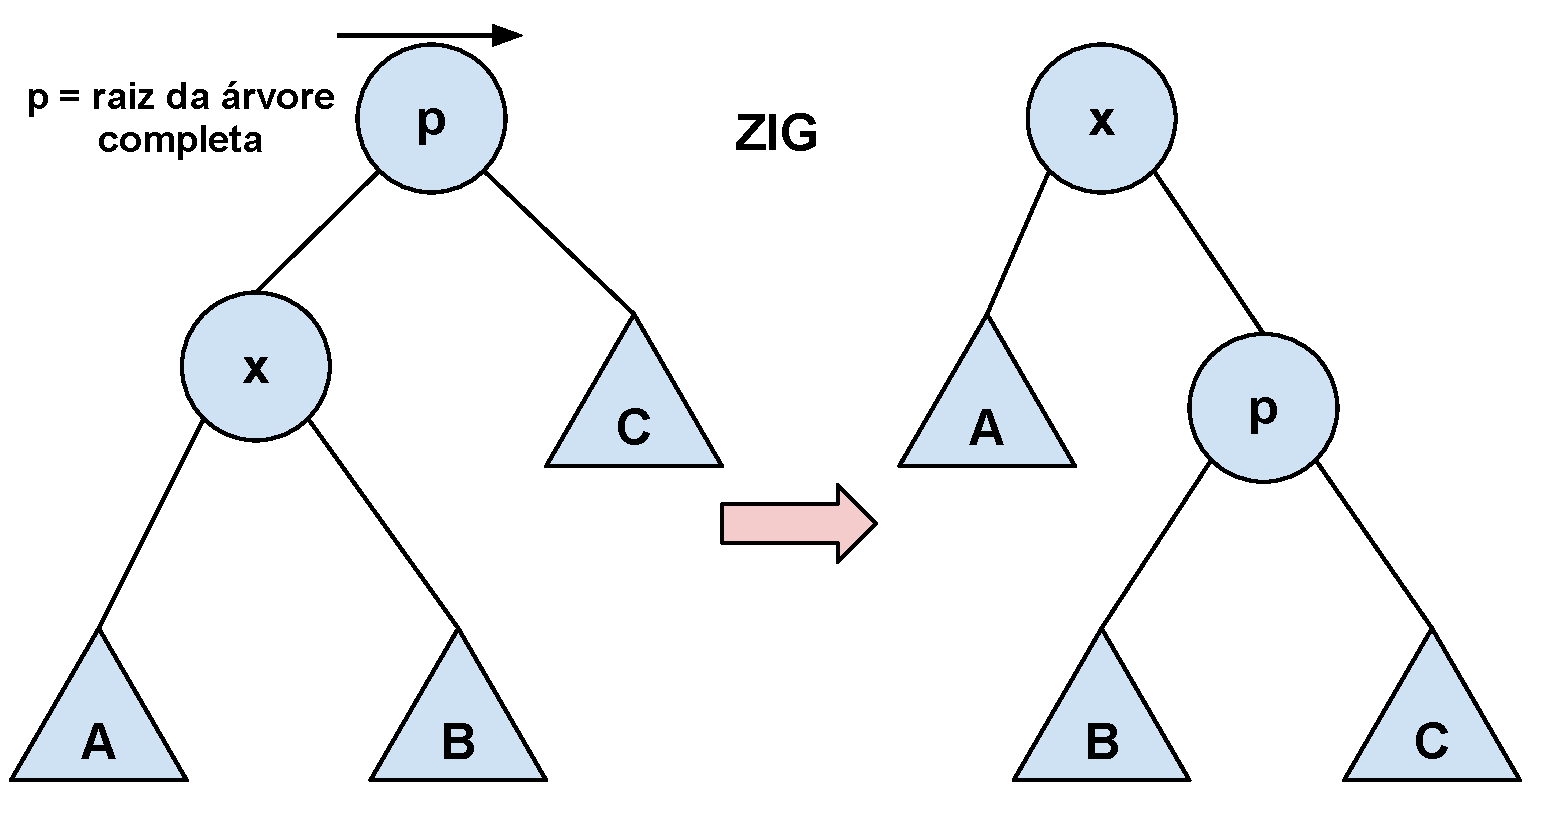
\includegraphics[keepaspectratio=true,width=4.5in]{figs/fig_arvores/Zig}
    \centering
    \end{figure}
}

%---------------------------------------------------------
\frame{
    \frametitle{Caso 2: ZIG-ZIG}
    
    \begin{figure}[tbp]
    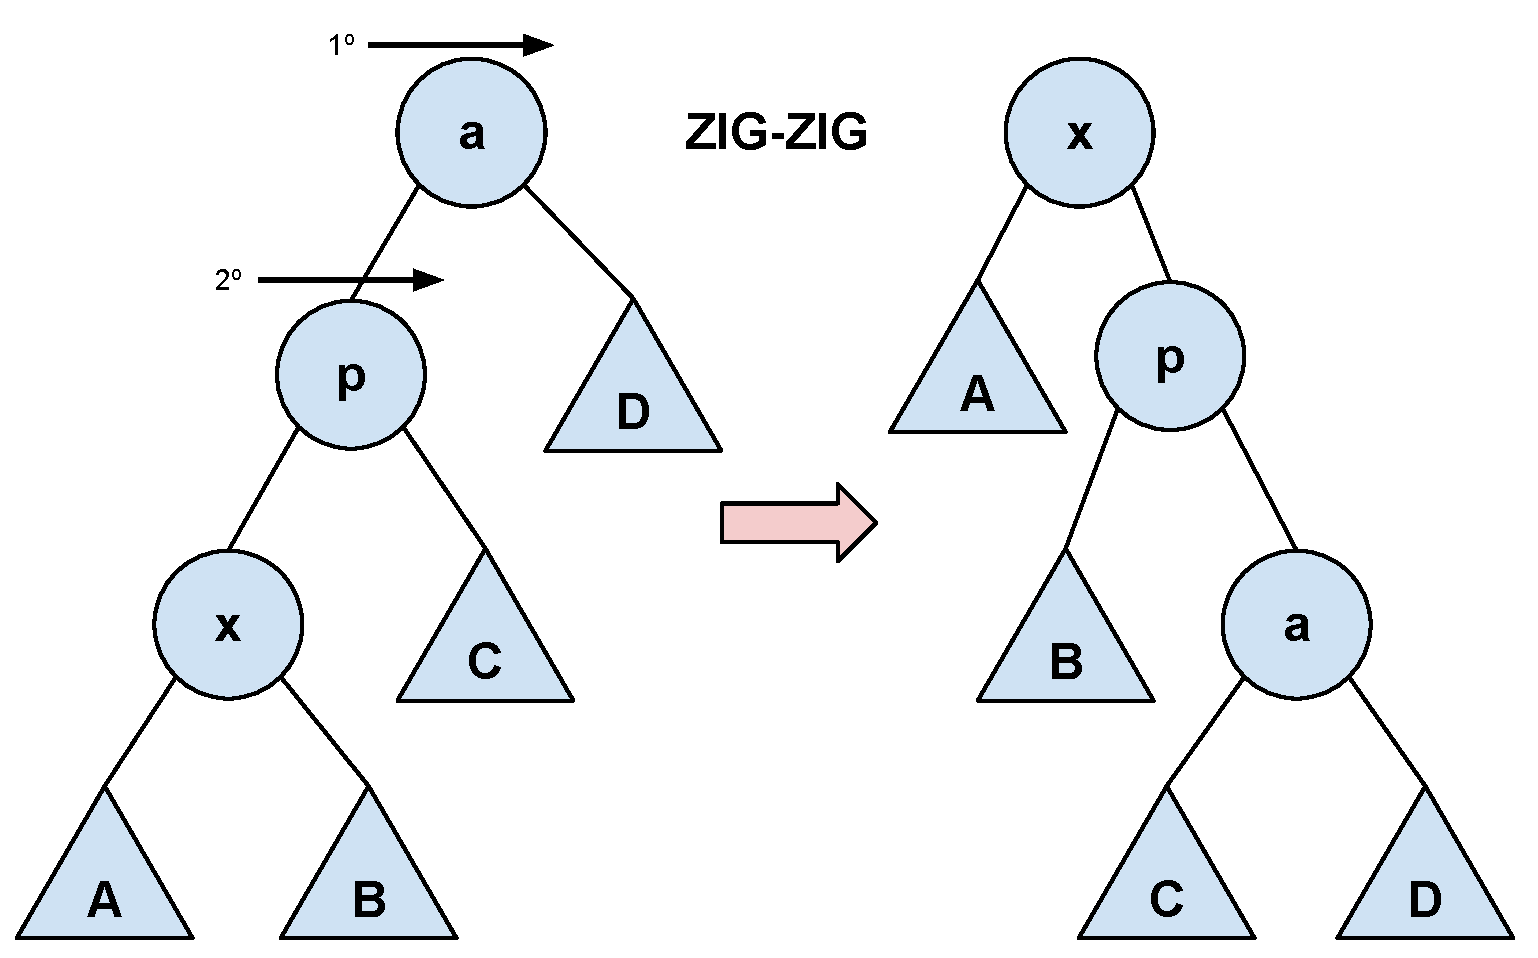
\includegraphics[keepaspectratio=true,width=4in]{figs/fig_arvores/Zig-Zig}
    \centering
    \end{figure}
}

%---------------------------------------------------------
\frame{
    \frametitle{Caso 3: ZIG-ZAG}
    
    \begin{figure}[tbp]
    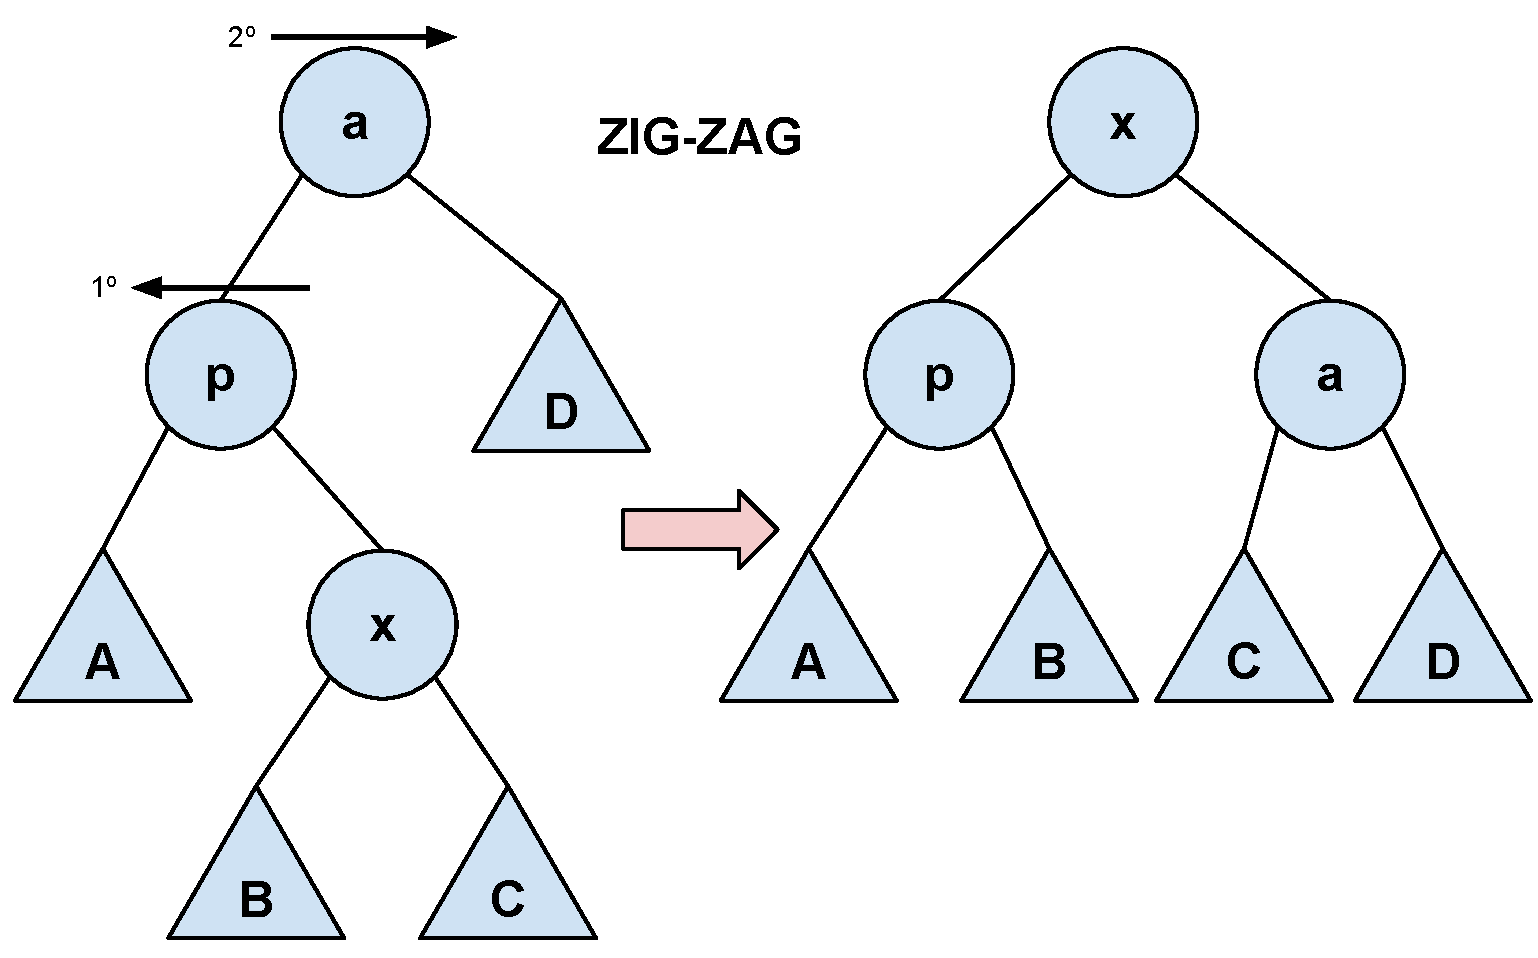
\includegraphics[keepaspectratio=true,width=4in]{figs/fig_arvores/Zig-Zag}
    \centering
    \end{figure}
}

%---------------------------------------------------------
\frame{
    \frametitle{Espalhamento Top-Down}
    
    \begin{itemize}
    \item Na estratégia Top-Down as chaves que estão no caminho da chave desejada
    para a raiz são rotacionadas e removidas para árvores auxiliares
    seguindo uma sequência de operações bem definidas
    \item Quando a chave desejada chega até a raiz, a árvore é remontada pelo
    retorno das chaves removidas
    \end{itemize}
}

%---------------------------------------------------------
\frame{
    \frametitle{Exemplo: Top-Down 1/6}
    
    \begin{figure}[tbp]
    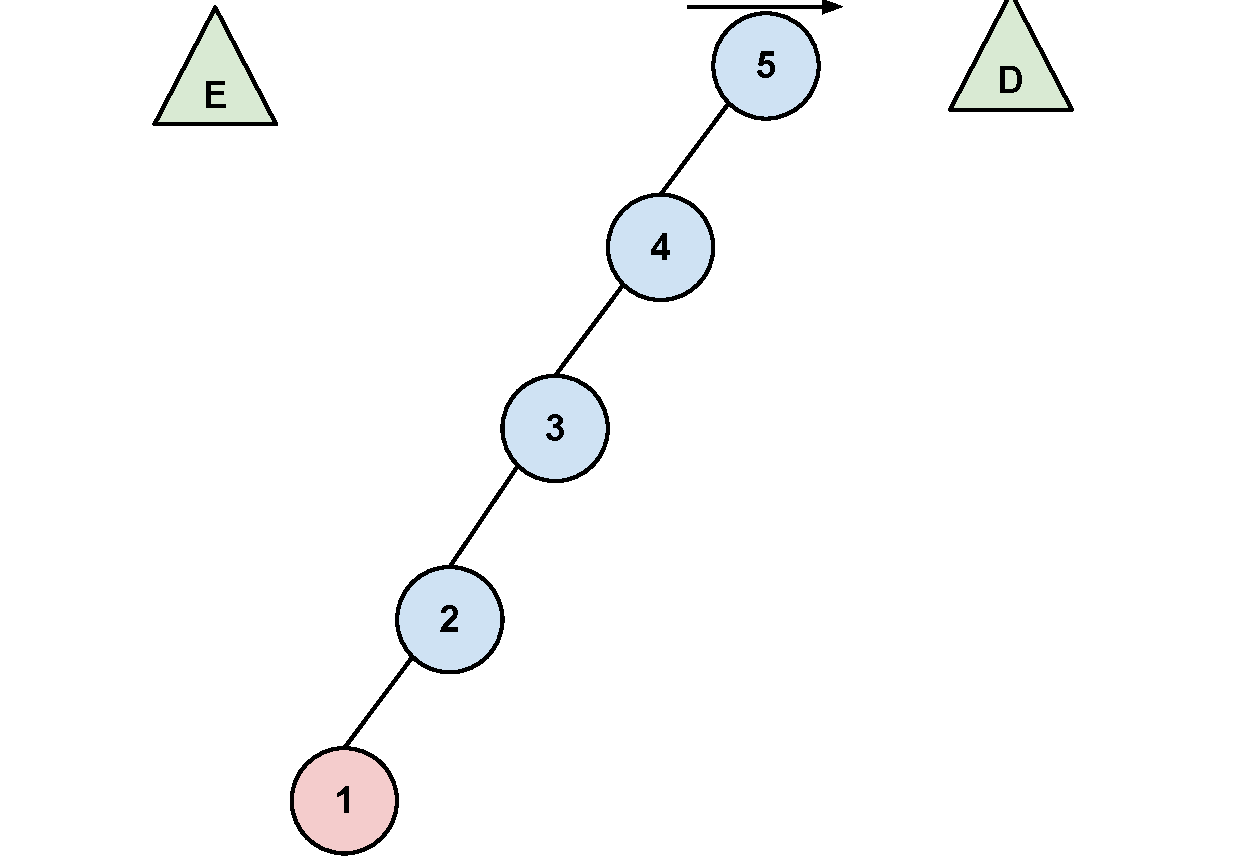
\includegraphics[keepaspectratio=true,width=3.5in]{figs/fig_arvores/Top-Down1}
    \centering
    \end{figure}
}

%---------------------------------------------------------
\frame{
    \frametitle{Exemplo: Top-Down 2/6}
    
    \begin{figure}[tbp]
    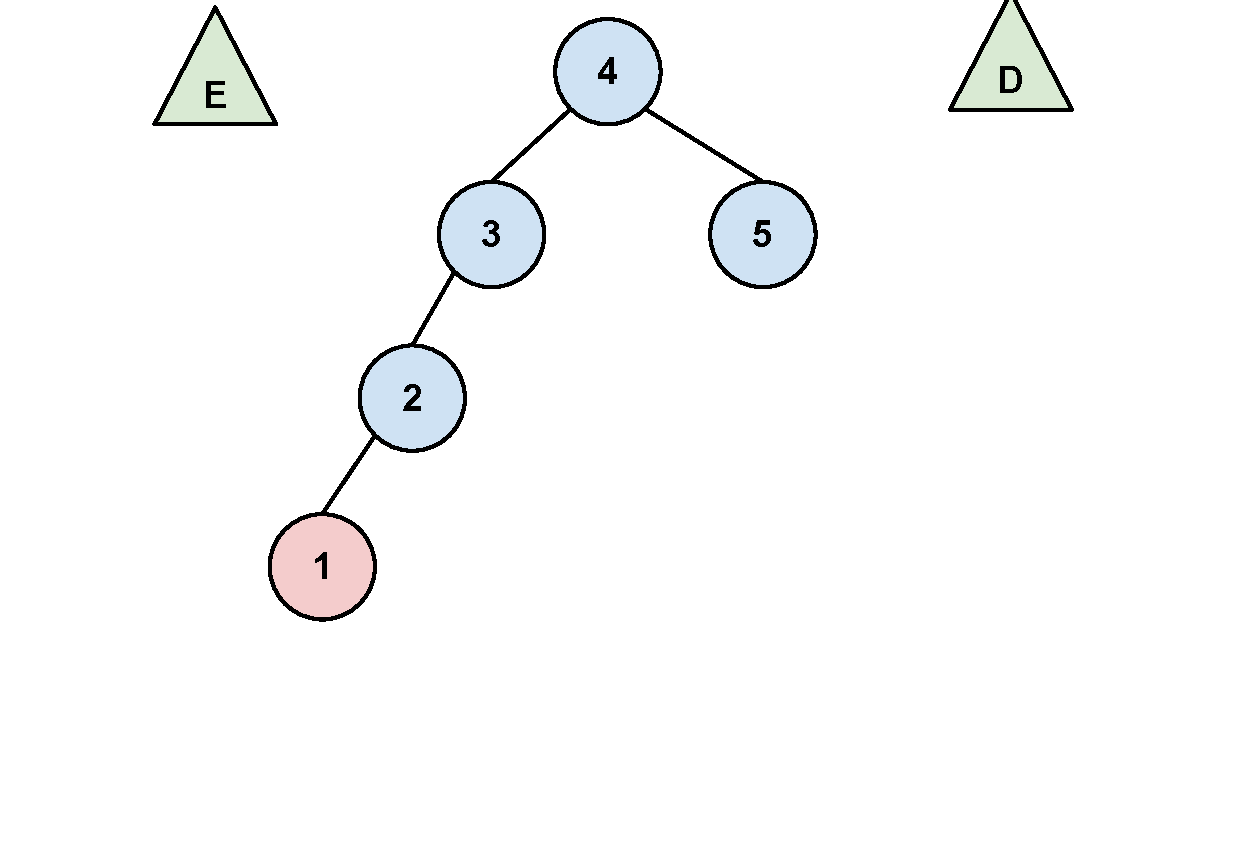
\includegraphics[keepaspectratio=true,width=3.5in]{figs/fig_arvores/Top-Down2}
    \centering
    \end{figure}
}

%---------------------------------------------------------
\frame{
    \frametitle{Exemplo: Top-Down 3/6}
    
    \begin{figure}[tbp]
    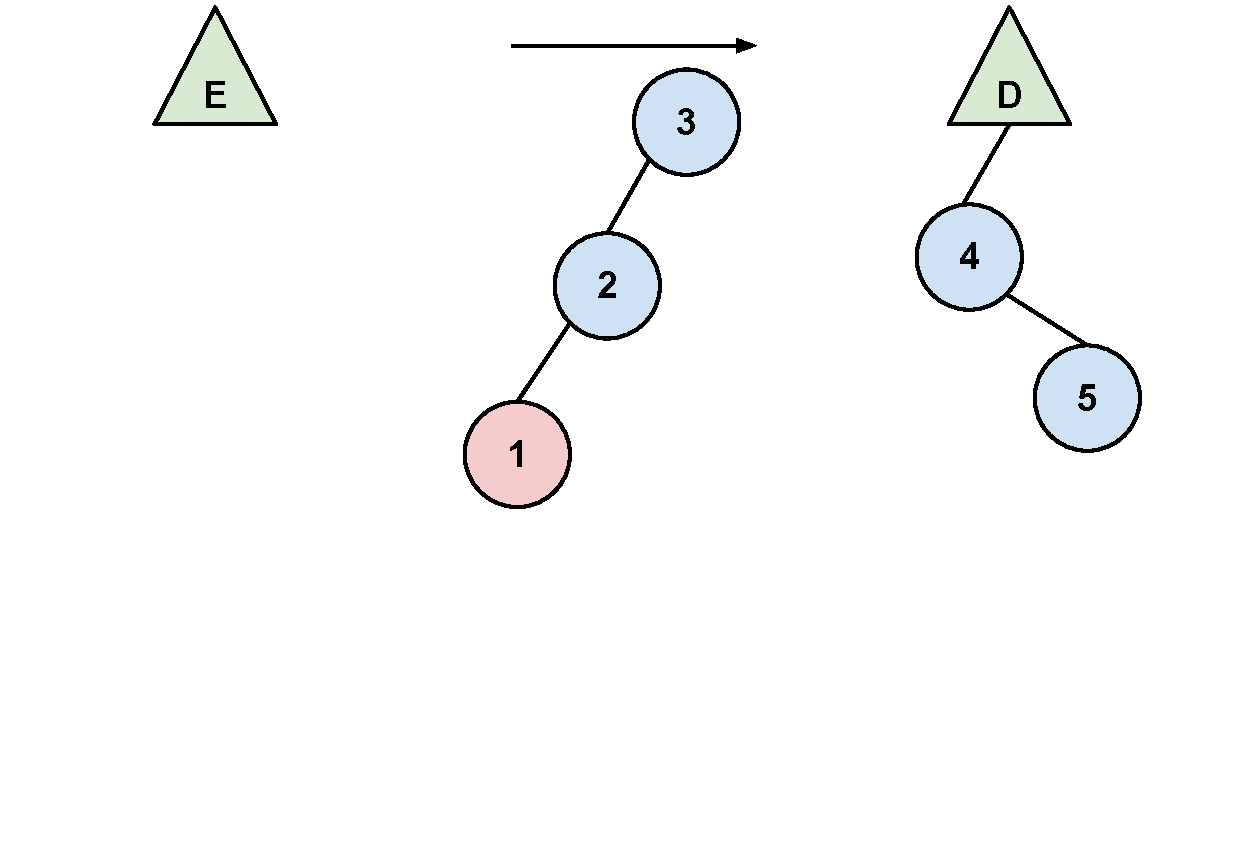
\includegraphics[keepaspectratio=true,width=3.5in]{figs/fig_arvores/Top-Down3}
    \centering
    \end{figure}
}

%---------------------------------------------------------
\frame{
    \frametitle{Exemplo: Top-Down 4/6}
    
    \begin{figure}[tbp]
    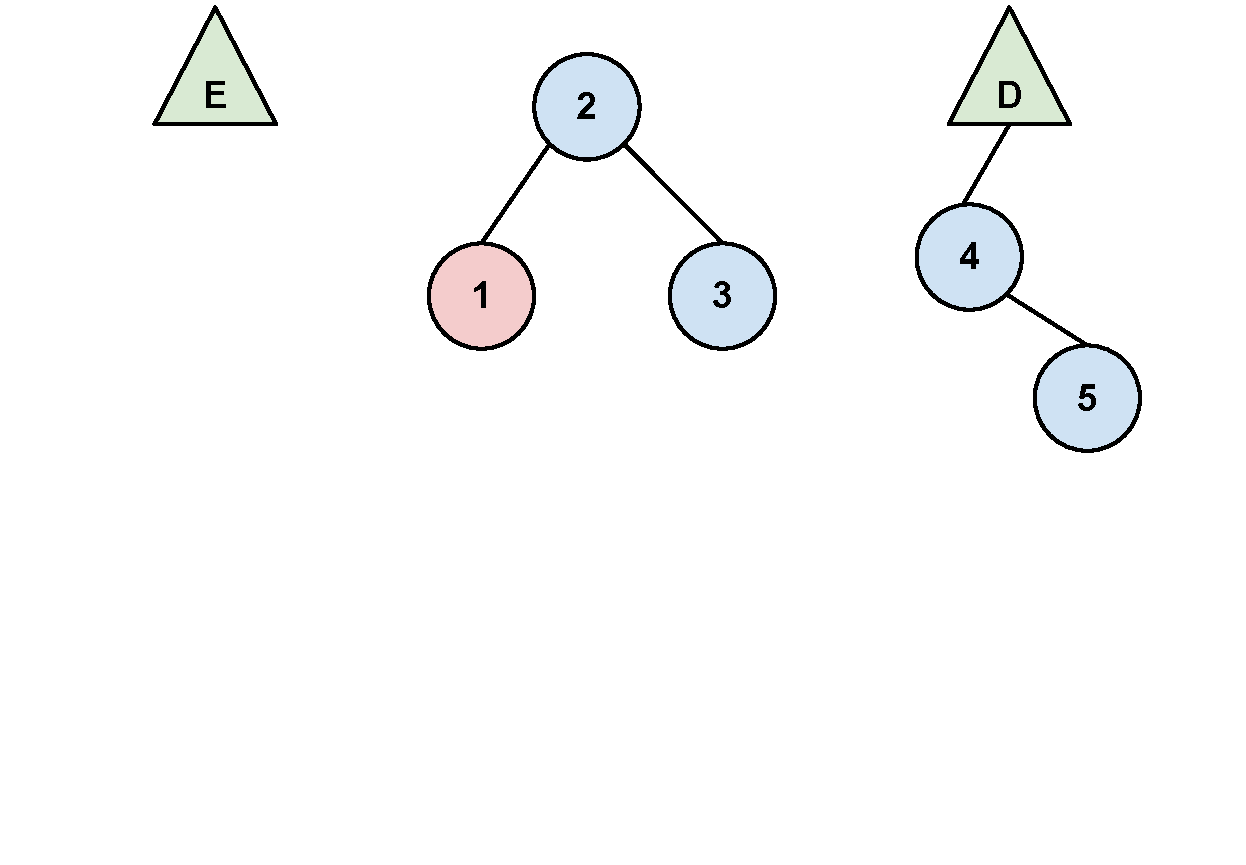
\includegraphics[keepaspectratio=true,width=3.5in]{figs/fig_arvores/Top-Down4}
    \centering
    \end{figure}
}

%---------------------------------------------------------
\frame{
    \frametitle{Exemplo: Top-Down 5/6}
    
    \begin{figure}[tbp]
    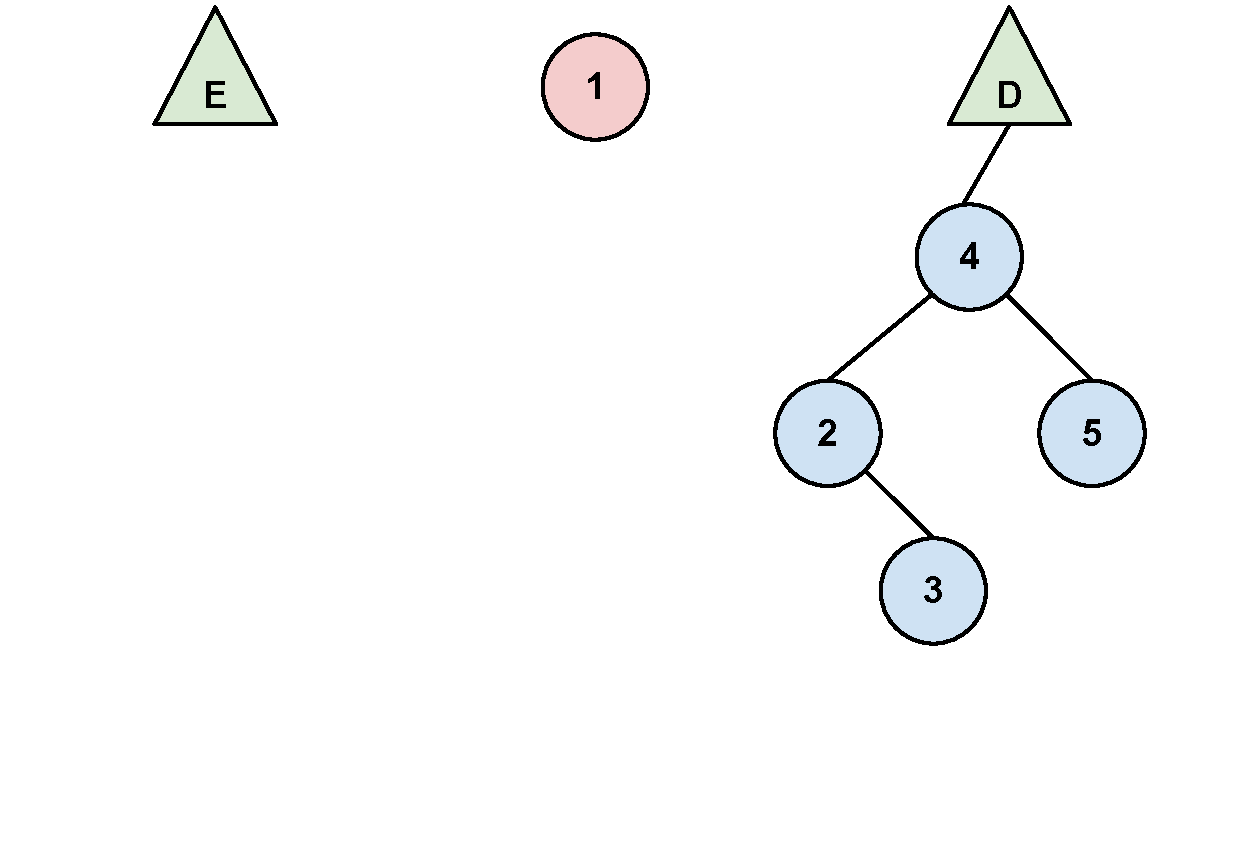
\includegraphics[keepaspectratio=true,width=3.5in]{figs/fig_arvores/Top-Down5}
    \centering
    \end{figure}
}

%---------------------------------------------------------
\frame{
    \frametitle{Exemplo: Top-Down 6/6}
    
    \begin{figure}[tbp]
    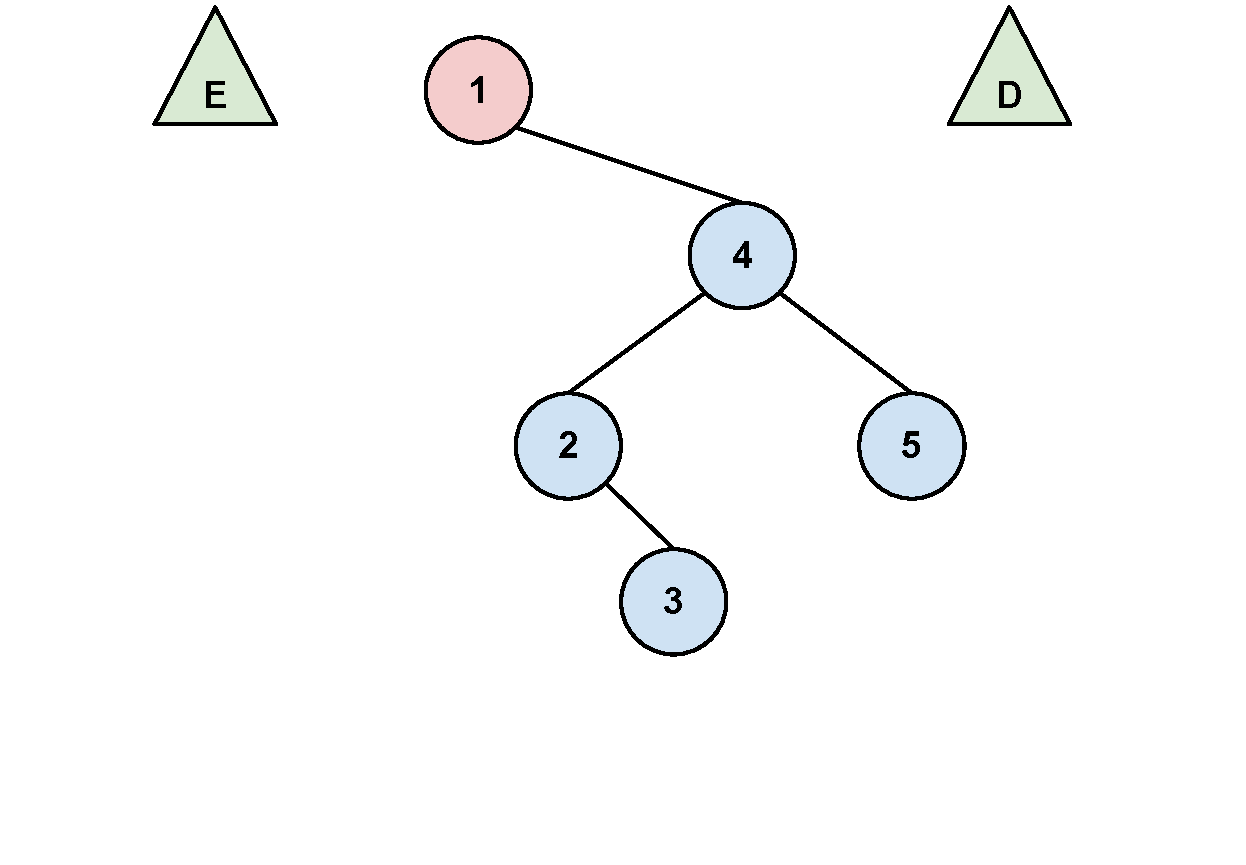
\includegraphics[keepaspectratio=true,width=3.5in]{figs/fig_arvores/Top-Down6}
    \centering
    \end{figure}
}




%---------------------------------------------------------
\begin{comment}
\section{Árvore B}

\bibliographystyle{unsrt}
\renewcommand\refname{Referências}

\frame{
    \frametitle{Referências}
    \bibliography{pres}
}

\end{comment}

%---------------------------------------------------------
 % cap 0

\end{document}
